\documentclass[1p]{elsarticle_modified}
%\bibliographystyle{elsarticle-num}

%\usepackage[colorlinks]{hyperref}
%\usepackage{abbrmath_seonhwa} %\Abb, \Ascr, \Acal ,\Abf, \Afrak
\usepackage{amsfonts}
\usepackage{amssymb}
\usepackage{amsmath}
\usepackage{amsthm}
\usepackage{scalefnt}
\usepackage{amsbsy}
\usepackage{kotex}
\usepackage{caption}
\usepackage{subfig}
\usepackage{color}
\usepackage{graphicx}
\usepackage{xcolor} %% white, black, red, green, blue, cyan, magenta, yellow
\usepackage{float}
\usepackage{setspace}
\usepackage{hyperref}

\usepackage{tikz}
\usetikzlibrary{arrows}

\usepackage{multirow}
\usepackage{array} % fixed length table
\usepackage{hhline}

%%%%%%%%%%%%%%%%%%%%%
\makeatletter
\renewcommand*\env@matrix[1][\arraystretch]{%
	\edef\arraystretch{#1}%
	\hskip -\arraycolsep
	\let\@ifnextchar\new@ifnextchar
	\array{*\c@MaxMatrixCols c}}
\makeatother %https://tex.stackexchange.com/questions/14071/how-can-i-increase-the-line-spacing-in-a-matrix
%%%%%%%%%%%%%%%

\usepackage[normalem]{ulem}

\newcommand{\msout}[1]{\ifmmode\text{\sout{\ensuremath{#1}}}\else\sout{#1}\fi}
%SOURCE: \msout is \stkout macro in https://tex.stackexchange.com/questions/20609/strikeout-in-math-mode

\newcommand{\cancel}[1]{
	\ifmmode
	{\color{red}\msout{#1}}
	\else
	{\color{red}\sout{#1}}
	\fi
}

\newcommand{\add}[1]{
	{\color{blue}\uwave{#1}}
}

\newcommand{\replace}[2]{
	\ifmmode
	{\color{red}\msout{#1}}{\color{blue}\uwave{#2}}
	\else
	{\color{red}\sout{#1}}{\color{blue}\uwave{#2}}
	\fi
}

\newcommand{\Sol}{\mathcal{S}} %segment
\newcommand{\D}{D} %diagram
\newcommand{\A}{\mathcal{A}} %arc


%%%%%%%%%%%%%%%%%%%%%%%%%%%%%5 test

\def\sl{\operatorname{\textup{SL}}(2,\Cbb)}
\def\psl{\operatorname{\textup{PSL}}(2,\Cbb)}
\def\quan{\mkern 1mu \triangleright \mkern 1mu}

\theoremstyle{definition}
\newtheorem{thm}{Theorem}[section]
\newtheorem{prop}[thm]{Proposition}
\newtheorem{lem}[thm]{Lemma}
\newtheorem{ques}[thm]{Question}
\newtheorem{cor}[thm]{Corollary}
\newtheorem{defn}[thm]{Definition}
\newtheorem{exam}[thm]{Example}
\newtheorem{rmk}[thm]{Remark}
\newtheorem{alg}[thm]{Algorithm}

\newcommand{\I}{\sqrt{-1}}
\begin{document}

%\begin{frontmatter}
%
%\title{Boundary parabolic representations of knots up to 8 crossings}
%
%%% Group authors per affiliation:
%\author{Yunhi Cho} 
%\address{Department of Mathematics, University of Seoul, Seoul, Korea}
%\ead{yhcho@uos.ac.kr}
%
%
%\author{Seonhwa Kim} %\fnref{s_kim}}
%\address{Center for Geometry and Physics, Institute for Basic Science, Pohang, 37673, Korea}
%\ead{ryeona17@ibs.re.kr}
%
%\author{Hyuk Kim}
%\address{Department of Mathematical Sciences, Seoul National University, Seoul 08826, Korea}
%\ead{hyukkim@snu.ac.kr}
%
%\author{Seokbeom Yoon}
%\address{Department of Mathematical Sciences, Seoul National University, Seoul, 08826,  Korea}
%\ead{sbyoon15@snu.ac.kr}
%
%\begin{abstract}
%We find all boundary parabolic representation of knots up to 8 crossings.
%
%\end{abstract}
%\begin{keyword}
%    \MSC[2010] 57M25 
%\end{keyword}
%
%\end{frontmatter}

%\linenumbers
%\tableofcontents
%
\newcommand\colored[1]{\textcolor{white}{\rule[-0.35ex]{0.8em}{1.4ex}}\kern-0.8em\color{red} #1}%
%\newcommand\colored[1]{\textcolor{white}{ #1}\kern-2.17ex	\textcolor{white}{ #1}\kern-1.81ex	\textcolor{white}{ #1}\kern-2.15ex\color{red}#1	}

{\Large $\underline{12a_{0387}~(K12a_{0387})}$}

\setlength{\tabcolsep}{10pt}
\renewcommand{\arraystretch}{1.6}
\vspace{1cm}\begin{tabular}{m{100pt}>{\centering\arraybackslash}m{274pt}}
\multirow{5}{120pt}{
	\centering
	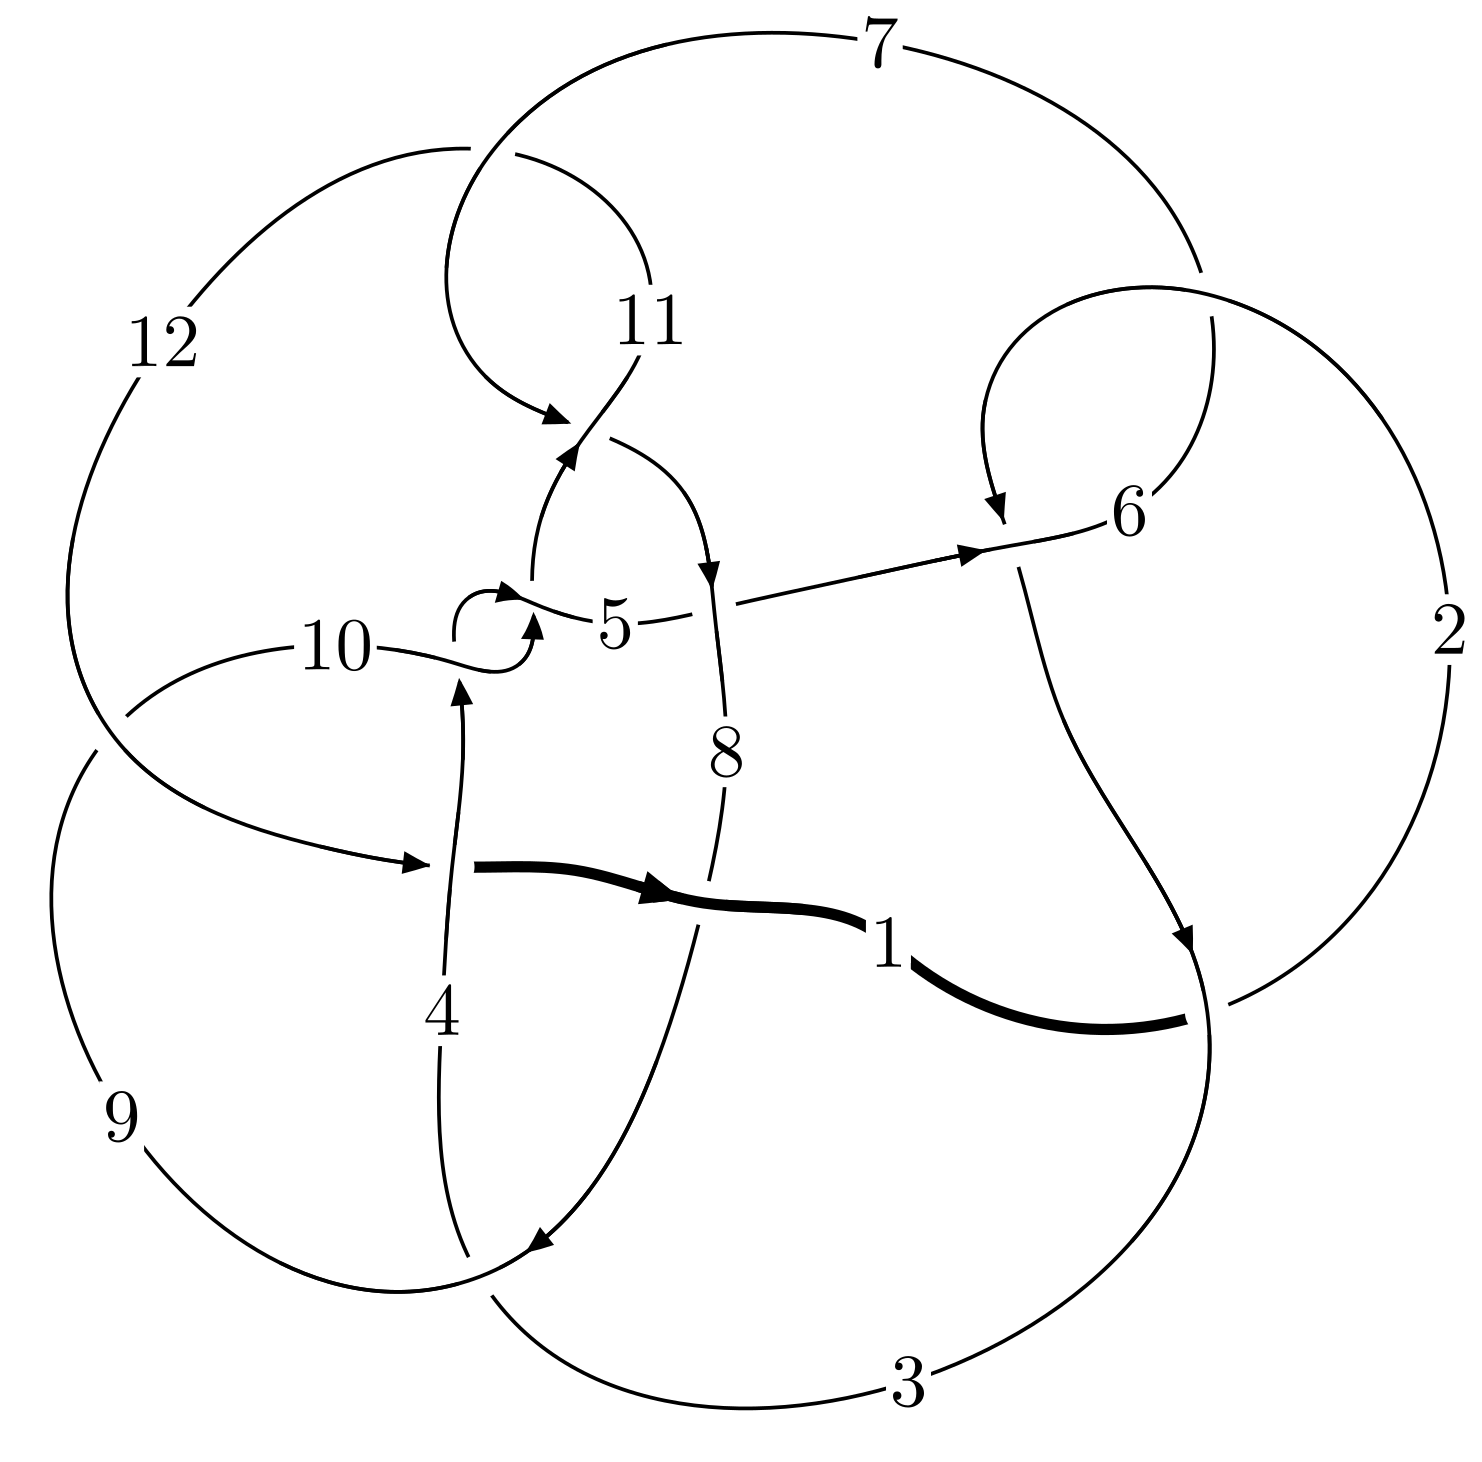
\includegraphics[width=112pt]{../../../GIT/diagram.site/Diagrams/png/1188_12a_0387.png}\\
\ \ \ A knot diagram\footnotemark}&
\allowdisplaybreaks
\textbf{Linearized knot diagam} \\
\cline{2-2}
 &
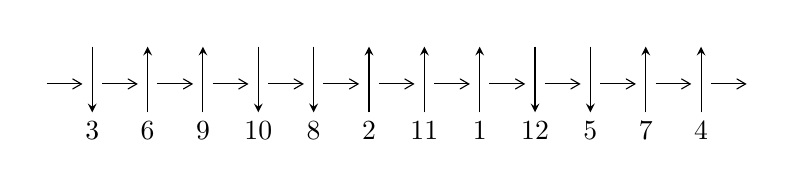
\begin{tikzpicture}[x=20pt, y=17pt]
	% nodes
	\node (C0) at (0, 0) {};
	\node (C1) at (1, 0) {};
	\node (C1U) at (1, +1) {};
	\node (C1D) at (1, -1) {3};

	\node (C2) at (2, 0) {};
	\node (C2U) at (2, +1) {};
	\node (C2D) at (2, -1) {6};

	\node (C3) at (3, 0) {};
	\node (C3U) at (3, +1) {};
	\node (C3D) at (3, -1) {9};

	\node (C4) at (4, 0) {};
	\node (C4U) at (4, +1) {};
	\node (C4D) at (4, -1) {10};

	\node (C5) at (5, 0) {};
	\node (C5U) at (5, +1) {};
	\node (C5D) at (5, -1) {8};

	\node (C6) at (6, 0) {};
	\node (C6U) at (6, +1) {};
	\node (C6D) at (6, -1) {2};

	\node (C7) at (7, 0) {};
	\node (C7U) at (7, +1) {};
	\node (C7D) at (7, -1) {11};

	\node (C8) at (8, 0) {};
	\node (C8U) at (8, +1) {};
	\node (C8D) at (8, -1) {1};

	\node (C9) at (9, 0) {};
	\node (C9U) at (9, +1) {};
	\node (C9D) at (9, -1) {12};

	\node (C10) at (10, 0) {};
	\node (C10U) at (10, +1) {};
	\node (C10D) at (10, -1) {5};

	\node (C11) at (11, 0) {};
	\node (C11U) at (11, +1) {};
	\node (C11D) at (11, -1) {7};

	\node (C12) at (12, 0) {};
	\node (C12U) at (12, +1) {};
	\node (C12D) at (12, -1) {4};
	\node (C13) at (13, 0) {};

	% arrows
	\draw[->,>={angle 60}]
	(C0) edge (C1) (C1) edge (C2) (C2) edge (C3) (C3) edge (C4) (C4) edge (C5) (C5) edge (C6) (C6) edge (C7) (C7) edge (C8) (C8) edge (C9) (C9) edge (C10) (C10) edge (C11) (C11) edge (C12) (C12) edge (C13) ;	\draw[->,>=stealth]
	(C1U) edge (C1D) (C2D) edge (C2U) (C3D) edge (C3U) (C4U) edge (C4D) (C5U) edge (C5D) (C6D) edge (C6U) (C7D) edge (C7U) (C8D) edge (C8U) (C9U) edge (C9D) (C10U) edge (C10D) (C11D) edge (C11U) (C12D) edge (C12U) ;
	\end{tikzpicture} \\
\hhline{~~} \\& 
\textbf{Solving Sequence} \\ \cline{2-2} 
 &
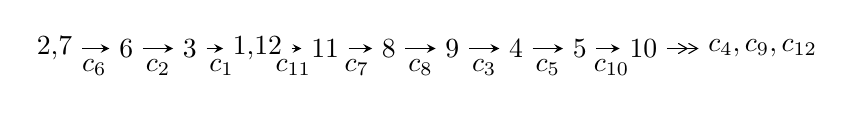
\begin{tikzpicture}[x=23pt, y=7pt]
	% node
	\node (A0) at (-1/8, 0) {2,7};
	\node (A1) at (1, 0) {6};
	\node (A2) at (2, 0) {3};
	\node (A3) at (49/16, 0) {1,12};
	\node (A4) at (33/8, 0) {11};
	\node (A5) at (41/8, 0) {8};
	\node (A6) at (49/8, 0) {9};
	\node (A7) at (57/8, 0) {4};
	\node (A8) at (65/8, 0) {5};
	\node (A9) at (73/8, 0) {10};
	\node (C1) at (1/2, -1) {$c_{6}$};
	\node (C2) at (3/2, -1) {$c_{2}$};
	\node (C3) at (5/2, -1) {$c_{1}$};
	\node (C4) at (29/8, -1) {$c_{11}$};
	\node (C5) at (37/8, -1) {$c_{7}$};
	\node (C6) at (45/8, -1) {$c_{8}$};
	\node (C7) at (53/8, -1) {$c_{3}$};
	\node (C8) at (61/8, -1) {$c_{5}$};
	\node (C9) at (69/8, -1) {$c_{10}$};
	\node (A10) at (11, 0) {$c_{4},c_{9},c_{12}$};

	% edge
	\draw[->,>=stealth]	
	(A0) edge (A1) (A1) edge (A2) (A2) edge (A3) (A3) edge (A4) (A4) edge (A5) (A5) edge (A6) (A6) edge (A7) (A7) edge (A8) (A8) edge (A9) ;
	\draw[->>,>={angle 60}]	
	(A9) edge (A10);
\end{tikzpicture} \\ 

\end{tabular} \\

\footnotetext{
The image of knot diagram is generated by the software ``\textbf{Draw programme}" developed by Andrew Bartholomew(\url{http://www.layer8.co.uk/maths/draw/index.htm\#Running-draw}), where we modified some parts for our purpose(\url{https://github.com/CATsTAILs/LinksPainter}).
}\phantom \\ \newline 
\centering \textbf{Ideals for irreducible components\footnotemark of $X_{\text{par}}$} 
 
\begin{align*}
I^u_{1}&=\langle 
-1.05426\times10^{408} u^{149}+3.71855\times10^{408} u^{148}+\cdots+2.44889\times10^{408} b+3.85948\times10^{410},\\
\phantom{I^u_{1}}&\phantom{= \langle  }-9.91717\times10^{409} u^{149}+3.49642\times10^{410} u^{148}+\cdots+1.29791\times10^{410} a+9.21565\times10^{412},\\
\phantom{I^u_{1}}&\phantom{= \langle  }u^{150}-4 u^{149}+\cdots-3712 u+424\rangle \\
I^u_{2}&=\langle 
4985116807 u^{41}-10536935014 u^{40}+\cdots+1443471113 b-1825302319,\\
\phantom{I^u_{2}}&\phantom{= \langle  }-2939589314 u^{41}+8863014375 u^{40}+\cdots+1443471113 a+1681161226,\\
\phantom{I^u_{2}}&\phantom{= \langle  }u^{42}-2 u^{41}+\cdots+8 u^2+1\rangle \\
I^u_{3}&=\langle 
-63975 a^5 u+71430 a^4 u+\cdots-875339 a-403473,\\
\phantom{I^u_{3}}&\phantom{= \langle  }a^6-3 a^5 u-4 a^5-4 a^4 u-7 a^4+41 a^3 u+16 a^3-35 a^2 u+19 a^2-8 a u-19 a+7 u-5,\;u^2+u+1\rangle \\
I^u_{4}&=\langle 
b+u+1,\;a+u+2,\;u^2+u+1\rangle \\
\\
\end{align*}
\raggedright * 4 irreducible components of $\dim_{\mathbb{C}}=0$, with total 206 representations.\\
\footnotetext{All coefficients of polynomials are rational numbers. But the coefficients are sometimes approximated in decimal forms when there is not enough margin.}
\newpage
\renewcommand{\arraystretch}{1}
\centering \section*{I. $I^u_{1}= \langle -1.05\times10^{408} u^{149}+3.72\times10^{408} u^{148}+\cdots+2.45\times10^{408} b+3.86\times10^{410},\;-9.92\times10^{409} u^{149}+3.50\times10^{410} u^{148}+\cdots+1.30\times10^{410} a+9.22\times10^{412},\;u^{150}-4 u^{149}+\cdots-3712 u+424 \rangle$}
\flushleft \textbf{(i) Arc colorings}\\
\begin{tabular}{m{7pt} m{180pt} m{7pt} m{180pt} }
\flushright $a_{2}=$&$\begin{pmatrix}0\\u\end{pmatrix}$ \\
\flushright $a_{7}=$&$\begin{pmatrix}1\\0\end{pmatrix}$ \\
\flushright $a_{6}=$&$\begin{pmatrix}1\\u^2\end{pmatrix}$ \\
\flushright $a_{3}=$&$\begin{pmatrix}u\\u^3+u\end{pmatrix}$ \\
\flushright $a_{1}=$&$\begin{pmatrix}u^3\\u^5+u^3+u\end{pmatrix}$ \\
\flushright $a_{12}=$&$\begin{pmatrix}0.764087 u^{149}-2.69388 u^{148}+\cdots+5171.06 u-710.037\\0.430506 u^{149}-1.51846 u^{148}+\cdots+1279.29 u-157.601\end{pmatrix}$ \\
\flushright $a_{11}=$&$\begin{pmatrix}0.333581 u^{149}-1.17542 u^{148}+\cdots+3891.77 u-552.435\\0.430506 u^{149}-1.51846 u^{148}+\cdots+1279.29 u-157.601\end{pmatrix}$ \\
\flushright $a_{8}=$&$\begin{pmatrix}0.314943 u^{149}-2.08245 u^{148}+\cdots+6240.60 u-840.864\\-0.496159 u^{149}+1.65502 u^{148}+\cdots-532.595 u+2.94029\end{pmatrix}$ \\
\flushright $a_{9}=$&$\begin{pmatrix}-0.0170775 u^{149}-0.874147 u^{148}+\cdots+5648.81 u-793.205\\-0.197127 u^{149}+0.554592 u^{148}+\cdots+953.099 u-169.611\end{pmatrix}$ \\
\flushright $a_{4}=$&$\begin{pmatrix}-0.227733 u^{149}+0.363072 u^{148}+\cdots-256.972 u+20.5049\\0.000513385 u^{149}+0.280826 u^{148}+\cdots-1172.62 u+165.784\end{pmatrix}$ \\
\flushright $a_{5}=$&$\begin{pmatrix}0.520345 u^{149}-2.09639 u^{148}+\cdots+2703.19 u-367.651\\-0.0869827 u^{149}+0.484600 u^{148}+\cdots-1601.48 u+211.163\end{pmatrix}$ \\
\flushright $a_{10}=$&$\begin{pmatrix}0.285141 u^{149}-0.818613 u^{148}+\cdots+3065.62 u-383.741\\0.373127 u^{149}-1.54301 u^{148}+\cdots+2854.14 u-378.233\end{pmatrix}$\\&\end{tabular}
\flushleft \textbf{(ii) Obstruction class $= -1$}\\~\\
\flushleft \textbf{(iii) Cusp Shapes $= 2.85672 u^{149}-10.8672 u^{148}+\cdots+14010.5 u-1820.76$}\\~\\
\newpage\renewcommand{\arraystretch}{1}
\flushleft \textbf{(iv) u-Polynomials at the component}\newline \\
\begin{tabular}{m{50pt}|m{274pt}}
Crossings & \hspace{64pt}u-Polynomials at each crossing \\
\hline $$\begin{aligned}c_{1}\end{aligned}$$&$\begin{aligned}
&u^{150}+60 u^{149}+\cdots+4386912 u+179776
\end{aligned}$\\
\hline $$\begin{aligned}c_{2},c_{6}\end{aligned}$$&$\begin{aligned}
&u^{150}+4 u^{149}+\cdots+3712 u+424
\end{aligned}$\\
\hline $$\begin{aligned}c_{3}\end{aligned}$$&$\begin{aligned}
&u^{150}+u^{149}+\cdots+3141 u+999
\end{aligned}$\\
\hline $$\begin{aligned}c_{4},c_{10}\end{aligned}$$&$\begin{aligned}
&u^{150}- u^{149}+\cdots-106584 u+13207
\end{aligned}$\\
\hline $$\begin{aligned}c_{5}\end{aligned}$$&$\begin{aligned}
&u^{150}-5 u^{149}+\cdots-8572569048 u+1134809017
\end{aligned}$\\
\hline $$\begin{aligned}c_{7},c_{11}\end{aligned}$$&$\begin{aligned}
&u^{150}-3 u^{149}+\cdots+655668 u+223897
\end{aligned}$\\
\hline $$\begin{aligned}c_{8}\end{aligned}$$&$\begin{aligned}
&u^{150}-9 u^{149}+\cdots+12351 u+1427
\end{aligned}$\\
\hline $$\begin{aligned}c_{9}\end{aligned}$$&$\begin{aligned}
&u^{150}-17 u^{149}+\cdots-14918 u+1267
\end{aligned}$\\
\hline $$\begin{aligned}c_{12}\end{aligned}$$&$\begin{aligned}
&u^{150}+13 u^{149}+\cdots+14298 u+1369
\end{aligned}$\\
\hline
\end{tabular}\\~\\
\newpage\renewcommand{\arraystretch}{1}
\flushleft \textbf{(v) Riley Polynomials at the component}\newline \\
\begin{tabular}{m{50pt}|m{274pt}}
Crossings & \hspace{64pt}Riley Polynomials at each crossing \\
\hline $$\begin{aligned}c_{1}\end{aligned}$$&$\begin{aligned}
&y^{150}+52 y^{149}+\cdots+1711720099328 y+32319410176
\end{aligned}$\\
\hline $$\begin{aligned}c_{2},c_{6}\end{aligned}$$&$\begin{aligned}
&y^{150}+60 y^{149}+\cdots+4386912 y+179776
\end{aligned}$\\
\hline $$\begin{aligned}c_{3}\end{aligned}$$&$\begin{aligned}
&y^{150}-17 y^{149}+\cdots-155034567 y+998001
\end{aligned}$\\
\hline $$\begin{aligned}c_{4},c_{10}\end{aligned}$$&$\begin{aligned}
&y^{150}-125 y^{149}+\cdots+19096275918 y+174424849
\end{aligned}$\\
\hline $$\begin{aligned}c_{5}\end{aligned}$$&$\begin{aligned}
&y^{150}-35 y^{149}+\cdots-7.46\times10^{19} y+1.29\times10^{18}
\end{aligned}$\\
\hline $$\begin{aligned}c_{7},c_{11}\end{aligned}$$&$\begin{aligned}
&y^{150}+105 y^{149}+\cdots+298851072020 y+50129866609
\end{aligned}$\\
\hline $$\begin{aligned}c_{8}\end{aligned}$$&$\begin{aligned}
&y^{150}+y^{149}+\cdots-5825915 y+2036329
\end{aligned}$\\
\hline $$\begin{aligned}c_{9}\end{aligned}$$&$\begin{aligned}
&y^{150}-27 y^{149}+\cdots+113839242 y+1605289
\end{aligned}$\\
\hline $$\begin{aligned}c_{12}\end{aligned}$$&$\begin{aligned}
&y^{150}+27 y^{149}+\cdots+47287964 y+1874161
\end{aligned}$\\
\hline
\end{tabular}\\~\\
\newpage\flushleft \textbf{(vi) Complex Volumes and Cusp Shapes}
$$\begin{array}{c|c|c}  
\text{Solutions to }I^u_{1}& \I (\text{vol} + \sqrt{-1}CS) & \text{Cusp shape}\\
 \hline 
\begin{aligned}
u &= -0.650950 + 0.755793 I \\
a &= -0.44599 - 2.08696 I \\
b &= -0.411761 - 0.718357 I\end{aligned}
 & \phantom{-}0.99424 + 1.29069 I & \phantom{-0.000000 } 0 \\ \hline\begin{aligned}
u &= -0.650950 - 0.755793 I \\
a &= -0.44599 + 2.08696 I \\
b &= -0.411761 + 0.718357 I\end{aligned}
 & \phantom{-}0.99424 - 1.29069 I & \phantom{-0.000000 } 0 \\ \hline\begin{aligned}
u &= \phantom{-}0.621403 + 0.786918 I \\
a &= -0.856285 + 1.117390 I \\
b &= -0.999949 + 0.281513 I\end{aligned}
 & \phantom{-}3.39719 + 0.83657 I & \phantom{-0.000000 } 0 \\ \hline\begin{aligned}
u &= \phantom{-}0.621403 - 0.786918 I \\
a &= -0.856285 - 1.117390 I \\
b &= -0.999949 - 0.281513 I\end{aligned}
 & \phantom{-}3.39719 - 0.83657 I & \phantom{-0.000000 } 0 \\ \hline\begin{aligned}
u &= \phantom{-}0.114917 + 1.008940 I \\
a &= -0.382018 - 0.545706 I \\
b &= \phantom{-}0.610476 - 0.043028 I\end{aligned}
 & -6.67344 - 0.00875 I & \phantom{-0.000000 } 0 \\ \hline\begin{aligned}
u &= \phantom{-}0.114917 - 1.008940 I \\
a &= -0.382018 + 0.545706 I \\
b &= \phantom{-}0.610476 + 0.043028 I\end{aligned}
 & -6.67344 + 0.00875 I & \phantom{-0.000000 } 0 \\ \hline\begin{aligned}
u &= \phantom{-}0.831449 + 0.585500 I \\
a &= \phantom{-}1.275070 - 0.064925 I \\
b &= \phantom{-}0.713685 + 0.361887 I\end{aligned}
 & \phantom{-}3.76191 - 3.62939 I & \phantom{-0.000000 } 0 \\ \hline\begin{aligned}
u &= \phantom{-}0.831449 - 0.585500 I \\
a &= \phantom{-}1.275070 + 0.064925 I \\
b &= \phantom{-}0.713685 - 0.361887 I\end{aligned}
 & \phantom{-}3.76191 + 3.62939 I & \phantom{-0.000000 } 0 \\ \hline\begin{aligned}
u &= -0.825173 + 0.532123 I \\
a &= -0.102577 + 0.528319 I \\
b &= -0.151141 + 0.842921 I\end{aligned}
 & \phantom{-}0.161939 - 1.273430 I & \phantom{-0.000000 } 0 \\ \hline\begin{aligned}
u &= -0.825173 - 0.532123 I \\
a &= -0.102577 - 0.528319 I \\
b &= -0.151141 - 0.842921 I\end{aligned}
 & \phantom{-}0.161939 + 1.273430 I & \phantom{-0.000000 } 0\\
 \hline 
 \end{array}$$\newpage$$\begin{array}{c|c|c}  
\text{Solutions to }I^u_{1}& \I (\text{vol} + \sqrt{-1}CS) & \text{Cusp shape}\\
 \hline 
\begin{aligned}
u &= -0.726183 + 0.722324 I \\
a &= \phantom{-}0.873867 + 0.265574 I \\
b &= \phantom{-}0.757927 + 0.274626 I\end{aligned}
 & -0.967754 - 0.375779 I & \phantom{-0.000000 } 0 \\ \hline\begin{aligned}
u &= -0.726183 - 0.722324 I \\
a &= \phantom{-}0.873867 - 0.265574 I \\
b &= \phantom{-}0.757927 - 0.274626 I\end{aligned}
 & -0.967754 + 0.375779 I & \phantom{-0.000000 } 0 \\ \hline\begin{aligned}
u &= -0.824969 + 0.494654 I \\
a &= -1.98368 - 0.36932 I \\
b &= -1.143490 + 0.137954 I\end{aligned}
 & -0.56940 + 7.88106 I & \phantom{-0.000000 } 0 \\ \hline\begin{aligned}
u &= -0.824969 - 0.494654 I \\
a &= -1.98368 + 0.36932 I \\
b &= -1.143490 - 0.137954 I\end{aligned}
 & -0.56940 - 7.88106 I & \phantom{-0.000000 } 0 \\ \hline\begin{aligned}
u &= -0.831057 + 0.622360 I \\
a &= \phantom{-}1.48914 + 0.17063 I \\
b &= \phantom{-}0.681374 - 0.497323 I\end{aligned}
 & \phantom{-}3.40903 - 3.07032 I & \phantom{-0.000000 } 0 \\ \hline\begin{aligned}
u &= -0.831057 - 0.622360 I \\
a &= \phantom{-}1.48914 - 0.17063 I \\
b &= \phantom{-}0.681374 + 0.497323 I\end{aligned}
 & \phantom{-}3.40903 + 3.07032 I & \phantom{-0.000000 } 0 \\ \hline\begin{aligned}
u &= -0.774546 + 0.695772 I \\
a &= \phantom{-}0.109303 + 0.971349 I \\
b &= \phantom{-}0.012048 + 0.882612 I\end{aligned}
 & \phantom{-}0.266192 - 1.288680 I & \phantom{-0.000000 } 0 \\ \hline\begin{aligned}
u &= -0.774546 - 0.695772 I \\
a &= \phantom{-}0.109303 - 0.971349 I \\
b &= \phantom{-}0.012048 - 0.882612 I\end{aligned}
 & \phantom{-}0.266192 + 1.288680 I & \phantom{-0.000000 } 0 \\ \hline\begin{aligned}
u &= \phantom{-}0.290064 + 0.898956 I \\
a &= \phantom{-}1.44191 + 0.49857 I \\
b &= \phantom{-}0.560825 + 0.278835 I\end{aligned}
 & -2.66861 - 2.39206 I & \phantom{-0.000000 } 0 \\ \hline\begin{aligned}
u &= \phantom{-}0.290064 - 0.898956 I \\
a &= \phantom{-}1.44191 - 0.49857 I \\
b &= \phantom{-}0.560825 - 0.278835 I\end{aligned}
 & -2.66861 + 2.39206 I & \phantom{-0.000000 } 0\\
 \hline 
 \end{array}$$\newpage$$\begin{array}{c|c|c}  
\text{Solutions to }I^u_{1}& \I (\text{vol} + \sqrt{-1}CS) & \text{Cusp shape}\\
 \hline 
\begin{aligned}
u &= \phantom{-}0.713200 + 0.791127 I \\
a &= -2.62672 - 0.39456 I \\
b &= -0.659778 - 0.741783 I\end{aligned}
 & -0.14769 + 5.52578 I & \phantom{-0.000000 } 0 \\ \hline\begin{aligned}
u &= \phantom{-}0.713200 - 0.791127 I \\
a &= -2.62672 + 0.39456 I \\
b &= -0.659778 + 0.741783 I\end{aligned}
 & -0.14769 - 5.52578 I & \phantom{-0.000000 } 0 \\ \hline\begin{aligned}
u &= \phantom{-}0.582752 + 0.729911 I \\
a &= -0.659704 + 0.827879 I \\
b &= -0.631795 + 1.018940 I\end{aligned}
 & \phantom{-}1.27517 - 1.70404 I & \phantom{-0.000000 } 0 \\ \hline\begin{aligned}
u &= \phantom{-}0.582752 - 0.729911 I \\
a &= -0.659704 - 0.827879 I \\
b &= -0.631795 - 1.018940 I\end{aligned}
 & \phantom{-}1.27517 + 1.70404 I & \phantom{-0.000000 } 0 \\ \hline\begin{aligned}
u &= \phantom{-}0.985549 + 0.417985 I \\
a &= -0.75578 + 1.24311 I \\
b &= -0.54984 + 1.37863 I\end{aligned}
 & -1.71146 - 5.79968 I & \phantom{-0.000000 } 0 \\ \hline\begin{aligned}
u &= \phantom{-}0.985549 - 0.417985 I \\
a &= -0.75578 - 1.24311 I \\
b &= -0.54984 - 1.37863 I\end{aligned}
 & -1.71146 + 5.79968 I & \phantom{-0.000000 } 0 \\ \hline\begin{aligned}
u &= -0.275656 + 0.887326 I \\
a &= -1.57663 - 0.50483 I \\
b &= \phantom{-}0.31725 + 1.54240 I\end{aligned}
 & -6.73260 + 4.81037 I & \phantom{-0.000000 } 0 \\ \hline\begin{aligned}
u &= -0.275656 - 0.887326 I \\
a &= -1.57663 + 0.50483 I \\
b &= \phantom{-}0.31725 - 1.54240 I\end{aligned}
 & -6.73260 - 4.81037 I & \phantom{-0.000000 } 0 \\ \hline\begin{aligned}
u &= -0.061811 + 1.070180 I \\
a &= \phantom{-}0.456316 - 0.345619 I \\
b &= \phantom{-}0.506918 + 0.009288 I\end{aligned}
 & -2.42430 - 2.76345 I & \phantom{-0.000000 } 0 \\ \hline\begin{aligned}
u &= -0.061811 - 1.070180 I \\
a &= \phantom{-}0.456316 + 0.345619 I \\
b &= \phantom{-}0.506918 - 0.009288 I\end{aligned}
 & -2.42430 + 2.76345 I & \phantom{-0.000000 } 0\\
 \hline 
 \end{array}$$\newpage$$\begin{array}{c|c|c}  
\text{Solutions to }I^u_{1}& \I (\text{vol} + \sqrt{-1}CS) & \text{Cusp shape}\\
 \hline 
\begin{aligned}
u &= -0.041663 + 1.072690 I \\
a &= -0.29566 - 1.72481 I \\
b &= \phantom{-}0.243974 + 1.295210 I\end{aligned}
 & -10.69020 + 2.88193 I & \phantom{-0.000000 } 0 \\ \hline\begin{aligned}
u &= -0.041663 - 1.072690 I \\
a &= -0.29566 + 1.72481 I \\
b &= \phantom{-}0.243974 - 1.295210 I\end{aligned}
 & -10.69020 - 2.88193 I & \phantom{-0.000000 } 0 \\ \hline\begin{aligned}
u &= \phantom{-}0.531037 + 0.933853 I \\
a &= \phantom{-}1.148340 + 0.581571 I \\
b &= \phantom{-}0.288731 - 0.872686 I\end{aligned}
 & -1.47947 + 7.40469 I & \phantom{-0.000000 } 0 \\ \hline\begin{aligned}
u &= \phantom{-}0.531037 - 0.933853 I \\
a &= \phantom{-}1.148340 - 0.581571 I \\
b &= \phantom{-}0.288731 + 0.872686 I\end{aligned}
 & -1.47947 - 7.40469 I & \phantom{-0.000000 } 0 \\ \hline\begin{aligned}
u &= -0.722429 + 0.576440 I \\
a &= \phantom{-}0.749423 + 0.528782 I \\
b &= \phantom{-}0.428522 + 1.299240 I\end{aligned}
 & -5.52036 + 3.96191 I & \phantom{-0.000000 } 0 \\ \hline\begin{aligned}
u &= -0.722429 - 0.576440 I \\
a &= \phantom{-}0.749423 - 0.528782 I \\
b &= \phantom{-}0.428522 - 1.299240 I\end{aligned}
 & -5.52036 - 3.96191 I & \phantom{-0.000000 } 0 \\ \hline\begin{aligned}
u &= \phantom{-}0.383504 + 1.006110 I \\
a &= -0.611075 + 0.283529 I \\
b &= \phantom{-}0.51502 - 1.34591 I\end{aligned}
 & -8.29483 + 0.76226 I & \phantom{-0.000000 } 0 \\ \hline\begin{aligned}
u &= \phantom{-}0.383504 - 1.006110 I \\
a &= -0.611075 - 0.283529 I \\
b &= \phantom{-}0.51502 + 1.34591 I\end{aligned}
 & -8.29483 - 0.76226 I & \phantom{-0.000000 } 0 \\ \hline\begin{aligned}
u &= -0.588937 + 0.708986 I \\
a &= \phantom{-}0.397719 + 1.079340 I \\
b &= \phantom{-}0.65335 + 1.38329 I\end{aligned}
 & -3.99681 + 5.06430 I & \phantom{-0.000000 } 0 \\ \hline\begin{aligned}
u &= -0.588937 - 0.708986 I \\
a &= \phantom{-}0.397719 - 1.079340 I \\
b &= \phantom{-}0.65335 - 1.38329 I\end{aligned}
 & -3.99681 - 5.06430 I & \phantom{-0.000000 } 0\\
 \hline 
 \end{array}$$\newpage$$\begin{array}{c|c|c}  
\text{Solutions to }I^u_{1}& \I (\text{vol} + \sqrt{-1}CS) & \text{Cusp shape}\\
 \hline 
\begin{aligned}
u &= \phantom{-}0.493151 + 0.774656 I \\
a &= \phantom{-}1.58068 - 2.20767 I \\
b &= \phantom{-}0.022793 + 0.937822 I\end{aligned}
 & -0.91992 - 3.22167 I & \phantom{-0.000000 } 0 \\ \hline\begin{aligned}
u &= \phantom{-}0.493151 - 0.774656 I \\
a &= \phantom{-}1.58068 + 2.20767 I \\
b &= \phantom{-}0.022793 - 0.937822 I\end{aligned}
 & -0.91992 + 3.22167 I & \phantom{-0.000000 } 0 \\ \hline\begin{aligned}
u &= \phantom{-}0.978308 + 0.473054 I \\
a &= \phantom{-}0.739734 - 0.456668 I \\
b &= \phantom{-}0.444904 - 1.083800 I\end{aligned}
 & \phantom{-}1.55723 - 8.02675 I & \phantom{-0.000000 } 0 \\ \hline\begin{aligned}
u &= \phantom{-}0.978308 - 0.473054 I \\
a &= \phantom{-}0.739734 + 0.456668 I \\
b &= \phantom{-}0.444904 + 1.083800 I\end{aligned}
 & \phantom{-}1.55723 + 8.02675 I & \phantom{-0.000000 } 0 \\ \hline\begin{aligned}
u &= \phantom{-}0.494537 + 0.967703 I \\
a &= \phantom{-}2.47444 - 0.63695 I \\
b &= \phantom{-}0.789877 + 1.164020 I\end{aligned}
 & -7.72315 + 4.99312 I & \phantom{-0.000000 } 0 \\ \hline\begin{aligned}
u &= \phantom{-}0.494537 - 0.967703 I \\
a &= \phantom{-}2.47444 + 0.63695 I \\
b &= \phantom{-}0.789877 - 1.164020 I\end{aligned}
 & -7.72315 - 4.99312 I & \phantom{-0.000000 } 0 \\ \hline\begin{aligned}
u &= \phantom{-}0.621848 + 0.892751 I \\
a &= -1.43500 + 0.37567 I \\
b &= -0.983201 - 0.454241 I\end{aligned}
 & \phantom{-}3.06867 + 4.05325 I & \phantom{-0.000000 } 0 \\ \hline\begin{aligned}
u &= \phantom{-}0.621848 - 0.892751 I \\
a &= -1.43500 - 0.37567 I \\
b &= -0.983201 + 0.454241 I\end{aligned}
 & \phantom{-}3.06867 - 4.05325 I & \phantom{-0.000000 } 0 \\ \hline\begin{aligned}
u &= \phantom{-}0.757337 + 0.790337 I \\
a &= -0.46674 - 2.05983 I \\
b &= \phantom{-}0.034037 - 1.003050 I\end{aligned}
 & -1.13396 - 3.55942 I & \phantom{-0.000000 } 0 \\ \hline\begin{aligned}
u &= \phantom{-}0.757337 - 0.790337 I \\
a &= -0.46674 + 2.05983 I \\
b &= \phantom{-}0.034037 + 1.003050 I\end{aligned}
 & -1.13396 + 3.55942 I & \phantom{-0.000000 } 0\\
 \hline 
 \end{array}$$\newpage$$\begin{array}{c|c|c}  
\text{Solutions to }I^u_{1}& \I (\text{vol} + \sqrt{-1}CS) & \text{Cusp shape}\\
 \hline 
\begin{aligned}
u &= \phantom{-}0.592903 + 0.922265 I \\
a &= -2.14985 + 0.57649 I \\
b &= -0.559444 - 1.141470 I\end{aligned}
 & \phantom{-}0.68849 + 6.39957 I & \phantom{-0.000000 } 0 \\ \hline\begin{aligned}
u &= \phantom{-}0.592903 - 0.922265 I \\
a &= -2.14985 - 0.57649 I \\
b &= -0.559444 + 1.141470 I\end{aligned}
 & \phantom{-}0.68849 - 6.39957 I & \phantom{-0.000000 } 0 \\ \hline\begin{aligned}
u &= -0.977164 + 0.531187 I \\
a &= -0.927771 - 1.027930 I \\
b &= -0.58404 - 1.34138 I\end{aligned}
 & -4.4056 + 13.9896 I & \phantom{-0.000000 } 0 \\ \hline\begin{aligned}
u &= -0.977164 - 0.531187 I \\
a &= -0.927771 + 1.027930 I \\
b &= -0.58404 + 1.34138 I\end{aligned}
 & -4.4056 - 13.9896 I & \phantom{-0.000000 } 0 \\ \hline\begin{aligned}
u &= -0.585919 + 0.958362 I \\
a &= \phantom{-}2.24941 + 0.52148 I \\
b &= \phantom{-}0.64230 - 1.51457 I\end{aligned}
 & -4.78169 - 9.74906 I & \phantom{-0.000000 } 0 \\ \hline\begin{aligned}
u &= -0.585919 - 0.958362 I \\
a &= \phantom{-}2.24941 - 0.52148 I \\
b &= \phantom{-}0.64230 + 1.51457 I\end{aligned}
 & -4.78169 + 9.74906 I & \phantom{-0.000000 } 0 \\ \hline\begin{aligned}
u &= -0.625189 + 0.938877 I \\
a &= -1.98223 + 0.76413 I \\
b &= -0.533832 + 0.743511 I\end{aligned}
 & \phantom{-}0.41871 - 6.27820 I & \phantom{-0.000000 } 0 \\ \hline\begin{aligned}
u &= -0.625189 - 0.938877 I \\
a &= -1.98223 - 0.76413 I \\
b &= -0.533832 - 0.743511 I\end{aligned}
 & \phantom{-}0.41871 + 6.27820 I & \phantom{-0.000000 } 0 \\ \hline\begin{aligned}
u &= \phantom{-}0.810088 + 0.800939 I \\
a &= -0.223635 + 0.414429 I \\
b &= \phantom{-}0.066297 + 0.944285 I\end{aligned}
 & -4.87474 + 3.08619 I & \phantom{-0.000000 } 0 \\ \hline\begin{aligned}
u &= \phantom{-}0.810088 - 0.800939 I \\
a &= -0.223635 - 0.414429 I \\
b &= \phantom{-}0.066297 - 0.944285 I\end{aligned}
 & -4.87474 - 3.08619 I & \phantom{-0.000000 } 0\\
 \hline 
 \end{array}$$\newpage$$\begin{array}{c|c|c}  
\text{Solutions to }I^u_{1}& \I (\text{vol} + \sqrt{-1}CS) & \text{Cusp shape}\\
 \hline 
\begin{aligned}
u &= \phantom{-}0.540746 + 1.004720 I \\
a &= \phantom{-}0.604989 - 0.987701 I \\
b &= \phantom{-}0.926149 - 0.025919 I\end{aligned}
 & -4.31926 + 5.98167 I & \phantom{-0.000000 } 0 \\ \hline\begin{aligned}
u &= \phantom{-}0.540746 - 1.004720 I \\
a &= \phantom{-}0.604989 + 0.987701 I \\
b &= \phantom{-}0.926149 + 0.025919 I\end{aligned}
 & -4.31926 - 5.98167 I & \phantom{-0.000000 } 0 \\ \hline\begin{aligned}
u &= \phantom{-}0.413846 + 0.750680 I \\
a &= \phantom{-}0.70316 - 2.01829 I \\
b &= \phantom{-}0.722478 - 0.919669 I\end{aligned}
 & -6.90497 - 1.16927 I & \phantom{-0.000000 } 0 \\ \hline\begin{aligned}
u &= \phantom{-}0.413846 - 0.750680 I \\
a &= \phantom{-}0.70316 + 2.01829 I \\
b &= \phantom{-}0.722478 + 0.919669 I\end{aligned}
 & -6.90497 + 1.16927 I & \phantom{-0.000000 } 0 \\ \hline\begin{aligned}
u &= -0.272092 + 0.809969 I \\
a &= -1.040330 + 0.672728 I \\
b &= -0.496985 - 1.005560 I\end{aligned}
 & -1.90581 + 1.97647 I & \phantom{-0.000000 } 0 \\ \hline\begin{aligned}
u &= -0.272092 - 0.809969 I \\
a &= -1.040330 - 0.672728 I \\
b &= -0.496985 + 1.005560 I\end{aligned}
 & -1.90581 - 1.97647 I & \phantom{-0.000000 } 0 \\ \hline\begin{aligned}
u &= \phantom{-}0.136984 + 1.152860 I \\
a &= \phantom{-}0.753093 - 1.067520 I \\
b &= \phantom{-}0.133213 + 1.247890 I\end{aligned}
 & -6.51856 - 0.37911 I & \phantom{-0.000000 } 0 \\ \hline\begin{aligned}
u &= \phantom{-}0.136984 - 1.152860 I \\
a &= \phantom{-}0.753093 + 1.067520 I \\
b &= \phantom{-}0.133213 - 1.247890 I\end{aligned}
 & -6.51856 + 0.37911 I & \phantom{-0.000000 } 0 \\ \hline\begin{aligned}
u &= \phantom{-}0.713406 + 0.927737 I \\
a &= \phantom{-}1.21139 + 1.69226 I \\
b &= \phantom{-}0.138195 + 0.969854 I\end{aligned}
 & -1.56011 + 9.13779 I & \phantom{-0.000000 } 0 \\ \hline\begin{aligned}
u &= \phantom{-}0.713406 - 0.927737 I \\
a &= \phantom{-}1.21139 - 1.69226 I \\
b &= \phantom{-}0.138195 - 0.969854 I\end{aligned}
 & -1.56011 - 9.13779 I & \phantom{-0.000000 } 0\\
 \hline 
 \end{array}$$\newpage$$\begin{array}{c|c|c}  
\text{Solutions to }I^u_{1}& \I (\text{vol} + \sqrt{-1}CS) & \text{Cusp shape}\\
 \hline 
\begin{aligned}
u &= -0.061121 + 1.178270 I \\
a &= -0.509371 - 0.330189 I \\
b &= -1.229600 - 0.240758 I\end{aligned}
 & -6.31401 + 5.88115 I & \phantom{-0.000000 } 0 \\ \hline\begin{aligned}
u &= -0.061121 - 1.178270 I \\
a &= -0.509371 + 0.330189 I \\
b &= -1.229600 + 0.240758 I\end{aligned}
 & -6.31401 - 5.88115 I & \phantom{-0.000000 } 0 \\ \hline\begin{aligned}
u &= -0.809128 + 0.117810 I \\
a &= -1.05186 + 1.59195 I \\
b &= -0.38320 + 1.40861 I\end{aligned}
 & -5.90630 + 2.54128 I & \phantom{-0.000000 } 0 \\ \hline\begin{aligned}
u &= -0.809128 - 0.117810 I \\
a &= -1.05186 - 1.59195 I \\
b &= -0.38320 - 1.40861 I\end{aligned}
 & -5.90630 - 2.54128 I & \phantom{-0.000000 } 0 \\ \hline\begin{aligned}
u &= \phantom{-}0.765197 + 0.905133 I \\
a &= -1.20307 + 1.47877 I \\
b &= -0.758829 + 0.845689 I\end{aligned}
 & -0.465950 + 0.095991 I & \phantom{-0.000000 } 0 \\ \hline\begin{aligned}
u &= \phantom{-}0.765197 - 0.905133 I \\
a &= -1.20307 - 1.47877 I \\
b &= -0.758829 - 0.845689 I\end{aligned}
 & -0.465950 - 0.095991 I & \phantom{-0.000000 } 0 \\ \hline\begin{aligned}
u &= -0.711895 + 0.956815 I \\
a &= \phantom{-}0.932444 + 0.558381 I \\
b &= \phantom{-}0.626586 - 0.432443 I\end{aligned}
 & -1.65089 - 5.10684 I & \phantom{-0.000000 } 0 \\ \hline\begin{aligned}
u &= -0.711895 - 0.956815 I \\
a &= \phantom{-}0.932444 - 0.558381 I \\
b &= \phantom{-}0.626586 + 0.432443 I\end{aligned}
 & -1.65089 + 5.10684 I & \phantom{-0.000000 } 0 \\ \hline\begin{aligned}
u &= \phantom{-}1.136500 + 0.382656 I \\
a &= -0.613173 - 0.907338 I \\
b &= -0.274027 - 1.296790 I\end{aligned}
 & -5.20724 + 7.78112 I & \phantom{-0.000000 } 0 \\ \hline\begin{aligned}
u &= \phantom{-}1.136500 - 0.382656 I \\
a &= -0.613173 + 0.907338 I \\
b &= -0.274027 + 1.296790 I\end{aligned}
 & -5.20724 - 7.78112 I & \phantom{-0.000000 } 0\\
 \hline 
 \end{array}$$\newpage$$\begin{array}{c|c|c}  
\text{Solutions to }I^u_{1}& \I (\text{vol} + \sqrt{-1}CS) & \text{Cusp shape}\\
 \hline 
\begin{aligned}
u &= -1.074900 + 0.535039 I \\
a &= \phantom{-}0.572072 + 0.589261 I \\
b &= \phantom{-}0.347227 + 1.067570 I\end{aligned}
 & \phantom{-}1.63852 + 0.87299 I & \phantom{-0.000000 } 0 \\ \hline\begin{aligned}
u &= -1.074900 - 0.535039 I \\
a &= \phantom{-}0.572072 - 0.589261 I \\
b &= \phantom{-}0.347227 - 1.067570 I\end{aligned}
 & \phantom{-}1.63852 - 0.87299 I & \phantom{-0.000000 } 0 \\ \hline\begin{aligned}
u &= -0.723079 + 0.962153 I \\
a &= \phantom{-}1.38564 - 0.68408 I \\
b &= \phantom{-}0.189428 - 0.925376 I\end{aligned}
 & -0.48629 - 4.36459 I & \phantom{-0.000000 } 0 \\ \hline\begin{aligned}
u &= -0.723079 - 0.962153 I \\
a &= \phantom{-}1.38564 + 0.68408 I \\
b &= \phantom{-}0.189428 + 0.925376 I\end{aligned}
 & -0.48629 + 4.36459 I & \phantom{-0.000000 } 0 \\ \hline\begin{aligned}
u &= \phantom{-}0.192422 + 1.188850 I \\
a &= -0.304068 + 0.939254 I \\
b &= \phantom{-}0.341009 - 1.251710 I\end{aligned}
 & -10.67590 - 3.59088 I & \phantom{-0.000000 } 0 \\ \hline\begin{aligned}
u &= \phantom{-}0.192422 - 1.188850 I \\
a &= -0.304068 - 0.939254 I \\
b &= \phantom{-}0.341009 + 1.251710 I\end{aligned}
 & -10.67590 + 3.59088 I & \phantom{-0.000000 } 0 \\ \hline\begin{aligned}
u &= \phantom{-}0.595979 + 1.050260 I \\
a &= -1.252900 + 0.541350 I \\
b &= -0.139471 - 1.324330 I\end{aligned}
 & -3.60547 + 7.44738 I & \phantom{-0.000000 } 0 \\ \hline\begin{aligned}
u &= \phantom{-}0.595979 - 1.050260 I \\
a &= -1.252900 - 0.541350 I \\
b &= -0.139471 + 1.324330 I\end{aligned}
 & -3.60547 - 7.44738 I & \phantom{-0.000000 } 0 \\ \hline\begin{aligned}
u &= -0.647017 + 1.031450 I \\
a &= \phantom{-}2.09180 + 0.64795 I \\
b &= \phantom{-}0.42011 - 1.37358 I\end{aligned}
 & -6.85865 - 9.22521 I & \phantom{-0.000000 } 0 \\ \hline\begin{aligned}
u &= -0.647017 - 1.031450 I \\
a &= \phantom{-}2.09180 - 0.64795 I \\
b &= \phantom{-}0.42011 + 1.37358 I\end{aligned}
 & -6.85865 + 9.22521 I & \phantom{-0.000000 } 0\\
 \hline 
 \end{array}$$\newpage$$\begin{array}{c|c|c}  
\text{Solutions to }I^u_{1}& \I (\text{vol} + \sqrt{-1}CS) & \text{Cusp shape}\\
 \hline 
\begin{aligned}
u &= -0.468310 + 1.125850 I \\
a &= -0.998152 - 0.988097 I \\
b &= -0.271389 + 1.144420 I\end{aligned}
 & -3.70741 - 4.72354 I & \phantom{-0.000000 } 0 \\ \hline\begin{aligned}
u &= -0.468310 - 1.125850 I \\
a &= -0.998152 + 0.988097 I \\
b &= -0.271389 - 1.144420 I\end{aligned}
 & -3.70741 + 4.72354 I & \phantom{-0.000000 } 0 \\ \hline\begin{aligned}
u &= \phantom{-}0.581506 + 1.082150 I \\
a &= \phantom{-}2.05829 - 0.79525 I \\
b &= \phantom{-}0.515155 + 1.284370 I\end{aligned}
 & -8.11659 + 11.17000 I & \phantom{-0.000000 } 0 \\ \hline\begin{aligned}
u &= \phantom{-}0.581506 - 1.082150 I \\
a &= \phantom{-}2.05829 + 0.79525 I \\
b &= \phantom{-}0.515155 - 1.284370 I\end{aligned}
 & -8.11659 - 11.17000 I & \phantom{-0.000000 } 0 \\ \hline\begin{aligned}
u &= -0.502774 + 1.121860 I \\
a &= \phantom{-}0.832395 - 0.342287 I \\
b &= -0.26050 - 1.63306 I\end{aligned}
 & -8.82750 - 7.10674 I & \phantom{-0.000000 } 0 \\ \hline\begin{aligned}
u &= -0.502774 - 1.121860 I \\
a &= \phantom{-}0.832395 + 0.342287 I \\
b &= -0.26050 + 1.63306 I\end{aligned}
 & -8.82750 + 7.10674 I & \phantom{-0.000000 } 0 \\ \hline\begin{aligned}
u &= \phantom{-}0.666100 + 0.336129 I \\
a &= \phantom{-}1.046180 - 0.481645 I \\
b &= \phantom{-}0.477078 - 1.218250 I\end{aligned}
 & -6.09544 - 6.32924 I & \phantom{-0.000000 } 0 \\ \hline\begin{aligned}
u &= \phantom{-}0.666100 - 0.336129 I \\
a &= \phantom{-}1.046180 + 0.481645 I \\
b &= \phantom{-}0.477078 + 1.218250 I\end{aligned}
 & -6.09544 + 6.32924 I & \phantom{-0.000000 } 0 \\ \hline\begin{aligned}
u &= \phantom{-}0.680060 + 1.058250 I \\
a &= \phantom{-}0.652114 - 0.693106 I \\
b &= \phantom{-}0.811675 - 0.272700 I\end{aligned}
 & \phantom{-}2.32250 + 9.27951 I & \phantom{-0.000000 } 0 \\ \hline\begin{aligned}
u &= \phantom{-}0.680060 - 1.058250 I \\
a &= \phantom{-}0.652114 + 0.693106 I \\
b &= \phantom{-}0.811675 + 0.272700 I\end{aligned}
 & \phantom{-}2.32250 - 9.27951 I & \phantom{-0.000000 } 0\\
 \hline 
 \end{array}$$\newpage$$\begin{array}{c|c|c}  
\text{Solutions to }I^u_{1}& \I (\text{vol} + \sqrt{-1}CS) & \text{Cusp shape}\\
 \hline 
\begin{aligned}
u &= -0.693006 + 1.052260 I \\
a &= \phantom{-}0.772413 + 0.692159 I \\
b &= \phantom{-}0.793311 + 0.470919 I\end{aligned}
 & \phantom{-}2.08595 - 2.62528 I & \phantom{-0.000000 } 0 \\ \hline\begin{aligned}
u &= -0.693006 - 1.052260 I \\
a &= \phantom{-}0.772413 - 0.692159 I \\
b &= \phantom{-}0.793311 - 0.470919 I\end{aligned}
 & \phantom{-}2.08595 + 2.62528 I & \phantom{-0.000000 } 0 \\ \hline\begin{aligned}
u &= \phantom{-}0.618538 + 0.393981 I \\
a &= \phantom{-}0.557185 + 0.370260 I \\
b &= -0.141671 + 1.154780 I\end{aligned}
 & -1.88431 - 2.63251 I & \phantom{-0.000000 } 0 \\ \hline\begin{aligned}
u &= \phantom{-}0.618538 - 0.393981 I \\
a &= \phantom{-}0.557185 - 0.370260 I \\
b &= -0.141671 - 1.154780 I\end{aligned}
 & -1.88431 + 2.63251 I & \phantom{-0.000000 } 0 \\ \hline\begin{aligned}
u &= \phantom{-}0.536784 + 1.148870 I \\
a &= -1.11407 + 1.08513 I \\
b &= -1.52251 + 0.35434 I\end{aligned}
 & -0.09056 + 4.18471 I & \phantom{-0.000000 } 0 \\ \hline\begin{aligned}
u &= \phantom{-}0.536784 - 1.148870 I \\
a &= -1.11407 - 1.08513 I \\
b &= -1.52251 - 0.35434 I\end{aligned}
 & -0.09056 - 4.18471 I & \phantom{-0.000000 } 0 \\ \hline\begin{aligned}
u &= -1.261540 + 0.133024 I \\
a &= \phantom{-}0.197607 - 0.212360 I \\
b &= \phantom{-}0.035794 - 0.956224 I\end{aligned}
 & \phantom{-}0.868836 - 0.257459 I & \phantom{-0.000000 } 0 \\ \hline\begin{aligned}
u &= -1.261540 - 0.133024 I \\
a &= \phantom{-}0.197607 + 0.212360 I \\
b &= \phantom{-}0.035794 + 0.956224 I\end{aligned}
 & \phantom{-}0.868836 + 0.257459 I & \phantom{-0.000000 } 0 \\ \hline\begin{aligned}
u &= \phantom{-}0.761715 + 1.020310 I \\
a &= -1.42624 - 0.03076 I \\
b &= -0.024599 - 1.073280 I\end{aligned}
 & -5.56602 + 2.91772 I & \phantom{-0.000000 } 0 \\ \hline\begin{aligned}
u &= \phantom{-}0.761715 - 1.020310 I \\
a &= -1.42624 + 0.03076 I \\
b &= -0.024599 + 1.073280 I\end{aligned}
 & -5.56602 - 2.91772 I & \phantom{-0.000000 } 0\\
 \hline 
 \end{array}$$\newpage$$\begin{array}{c|c|c}  
\text{Solutions to }I^u_{1}& \I (\text{vol} + \sqrt{-1}CS) & \text{Cusp shape}\\
 \hline 
\begin{aligned}
u &= -0.651941 + 1.094300 I \\
a &= -1.13866 - 1.07029 I \\
b &= -1.300600 - 0.162937 I\end{aligned}
 & -2.36595 - 13.40950 I & \phantom{-0.000000 } 0 \\ \hline\begin{aligned}
u &= -0.651941 - 1.094300 I \\
a &= -1.13866 + 1.07029 I \\
b &= -1.300600 + 0.162937 I\end{aligned}
 & -2.36595 + 13.40950 I & \phantom{-0.000000 } 0 \\ \hline\begin{aligned}
u &= -0.280043 + 1.263290 I \\
a &= -1.152490 - 0.363033 I \\
b &= -0.64298 + 1.54653 I\end{aligned}
 & -10.36940 - 1.32994 I & \phantom{-0.000000 } 0 \\ \hline\begin{aligned}
u &= -0.280043 - 1.263290 I \\
a &= -1.152490 + 0.363033 I \\
b &= -0.64298 - 1.54653 I\end{aligned}
 & -10.36940 + 1.32994 I & \phantom{-0.000000 } 0 \\ \hline\begin{aligned}
u &= \phantom{-}0.087934 + 1.321040 I \\
a &= -0.485989 + 0.597999 I \\
b &= -0.44106 - 1.43842 I\end{aligned}
 & -11.7739 + 11.5393 I & \phantom{-0.000000 } 0 \\ \hline\begin{aligned}
u &= \phantom{-}0.087934 - 1.321040 I \\
a &= -0.485989 - 0.597999 I \\
b &= -0.44106 + 1.43842 I\end{aligned}
 & -11.7739 - 11.5393 I & \phantom{-0.000000 } 0 \\ \hline\begin{aligned}
u &= -0.788952 + 1.066170 I \\
a &= \phantom{-}0.556902 - 0.062106 I \\
b &= \phantom{-}0.051172 - 0.733929 I\end{aligned}
 & -1.44150 - 4.85210 I & \phantom{-0.000000 } 0 \\ \hline\begin{aligned}
u &= -0.788952 - 1.066170 I \\
a &= \phantom{-}0.556902 + 0.062106 I \\
b &= \phantom{-}0.051172 + 0.733929 I\end{aligned}
 & -1.44150 + 4.85210 I & \phantom{-0.000000 } 0 \\ \hline\begin{aligned}
u &= \phantom{-}0.693021 + 1.149290 I \\
a &= \phantom{-}1.67113 - 0.49046 I \\
b &= \phantom{-}0.484683 + 1.184340 I\end{aligned}
 & -0.52663 + 14.08750 I & \phantom{-0.000000 } 0 \\ \hline\begin{aligned}
u &= \phantom{-}0.693021 - 1.149290 I \\
a &= \phantom{-}1.67113 + 0.49046 I \\
b &= \phantom{-}0.484683 - 1.184340 I\end{aligned}
 & -0.52663 - 14.08750 I & \phantom{-0.000000 } 0\\
 \hline 
 \end{array}$$\newpage$$\begin{array}{c|c|c}  
\text{Solutions to }I^u_{1}& \I (\text{vol} + \sqrt{-1}CS) & \text{Cusp shape}\\
 \hline 
\begin{aligned}
u &= -0.714398 + 1.137700 I \\
a &= -2.04445 - 0.22489 I \\
b &= -0.63841 + 1.38263 I\end{aligned}
 & -6.2951 - 20.1515 I & \phantom{-0.000000 } 0 \\ \hline\begin{aligned}
u &= -0.714398 - 1.137700 I \\
a &= -2.04445 + 0.22489 I \\
b &= -0.63841 - 1.38263 I\end{aligned}
 & -6.2951 + 20.1515 I & \phantom{-0.000000 } 0 \\ \hline\begin{aligned}
u &= -0.725520 + 1.139120 I \\
a &= \phantom{-}1.65930 + 0.26547 I \\
b &= \phantom{-}0.450946 - 1.158360 I\end{aligned}
 & -0.29198 - 7.24361 I & \phantom{-0.000000 } 0 \\ \hline\begin{aligned}
u &= -0.725520 - 1.139120 I \\
a &= \phantom{-}1.65930 - 0.26547 I \\
b &= \phantom{-}0.450946 + 1.158360 I\end{aligned}
 & -0.29198 + 7.24361 I & \phantom{-0.000000 } 0 \\ \hline\begin{aligned}
u &= \phantom{-}0.684601 + 1.171970 I \\
a &= -1.90470 + 0.10444 I \\
b &= -0.68210 - 1.44306 I\end{aligned}
 & -4.01000 + 11.84820 I & \phantom{-0.000000 } 0 \\ \hline\begin{aligned}
u &= \phantom{-}0.684601 - 1.171970 I \\
a &= -1.90470 - 0.10444 I \\
b &= -0.68210 + 1.44306 I\end{aligned}
 & -4.01000 - 11.84820 I & \phantom{-0.000000 } 0 \\ \hline\begin{aligned}
u &= \phantom{-}0.536805 + 0.352824 I \\
a &= \phantom{-}1.153040 - 0.032500 I \\
b &= \phantom{-}0.785953 + 0.066946 I\end{aligned}
 & -2.69886 - 1.68877 I & \phantom{-0.000000 } 0 \\ \hline\begin{aligned}
u &= \phantom{-}0.536805 - 0.352824 I \\
a &= \phantom{-}1.153040 + 0.032500 I \\
b &= \phantom{-}0.785953 - 0.066946 I\end{aligned}
 & -2.69886 + 1.68877 I & \phantom{-0.000000 } 0 \\ \hline\begin{aligned}
u &= \phantom{-}0.525980 + 0.367283 I \\
a &= -1.45876 - 2.26168 I \\
b &= -0.313122 - 0.123679 I\end{aligned}
 & -0.68433 + 5.18324 I & \phantom{-}7.31593 - 7.24109 I \\ \hline\begin{aligned}
u &= \phantom{-}0.525980 - 0.367283 I \\
a &= -1.45876 + 2.26168 I \\
b &= -0.313122 + 0.123679 I\end{aligned}
 & -0.68433 - 5.18324 I & \phantom{-}7.31593 + 7.24109 I\\
 \hline 
 \end{array}$$\newpage$$\begin{array}{c|c|c}  
\text{Solutions to }I^u_{1}& \I (\text{vol} + \sqrt{-1}CS) & \text{Cusp shape}\\
 \hline 
\begin{aligned}
u &= \phantom{-}0.186049 + 0.608710 I \\
a &= \phantom{-}1.12188 - 0.95562 I \\
b &= -0.314400 + 1.060000 I\end{aligned}
 & -1.64492 - 2.67203 I & -4.50874 + 6.35714 I \\ \hline\begin{aligned}
u &= \phantom{-}0.186049 - 0.608710 I \\
a &= \phantom{-}1.12188 + 0.95562 I \\
b &= -0.314400 - 1.060000 I\end{aligned}
 & -1.64492 + 2.67203 I & -4.50874 - 6.35714 I \\ \hline\begin{aligned}
u &= -0.082572 + 1.370880 I \\
a &= \phantom{-}0.322643 + 0.757160 I \\
b &= \phantom{-}0.181283 - 1.141450 I\end{aligned}
 & -5.68035 - 5.08287 I & \phantom{-0.000000 } 0 \\ \hline\begin{aligned}
u &= -0.082572 - 1.370880 I \\
a &= \phantom{-}0.322643 - 0.757160 I \\
b &= \phantom{-}0.181283 + 1.141450 I\end{aligned}
 & -5.68035 + 5.08287 I & \phantom{-0.000000 } 0 \\ \hline\begin{aligned}
u &= \phantom{-}0.468808 + 0.378093 I \\
a &= -2.69092 + 1.38331 I \\
b &= -1.087480 - 0.243844 I\end{aligned}
 & \phantom{-}2.31321 + 0.20343 I & \phantom{-}4.06423 + 2.59642 I \\ \hline\begin{aligned}
u &= \phantom{-}0.468808 - 0.378093 I \\
a &= -2.69092 - 1.38331 I \\
b &= -1.087480 + 0.243844 I\end{aligned}
 & \phantom{-}2.31321 - 0.20343 I & \phantom{-}4.06423 - 2.59642 I \\ \hline\begin{aligned}
u &= -0.64713 + 1.27358 I \\
a &= -0.772154 - 0.487196 I \\
b &= -0.153719 + 1.035400 I\end{aligned}
 & -2.78167 - 5.98666 I & \phantom{-0.000000 } 0 \\ \hline\begin{aligned}
u &= -0.64713 - 1.27358 I \\
a &= -0.772154 + 0.487196 I \\
b &= -0.153719 - 1.035400 I\end{aligned}
 & -2.78167 + 5.98666 I & \phantom{-0.000000 } 0 \\ \hline\begin{aligned}
u &= \phantom{-}0.52603 + 1.32883 I \\
a &= \phantom{-}0.618820 + 0.111020 I \\
b &= -0.098842 + 1.403380 I\end{aligned}
 & -8.60944 - 1.41407 I & \phantom{-0.000000 } 0 \\ \hline\begin{aligned}
u &= \phantom{-}0.52603 - 1.32883 I \\
a &= \phantom{-}0.618820 - 0.111020 I \\
b &= -0.098842 - 1.403380 I\end{aligned}
 & -8.60944 + 1.41407 I & \phantom{-0.000000 } 0\\
 \hline 
 \end{array}$$\newpage$$\begin{array}{c|c|c}  
\text{Solutions to }I^u_{1}& \I (\text{vol} + \sqrt{-1}CS) & \text{Cusp shape}\\
 \hline 
\begin{aligned}
u &= -0.330520 + 0.429626 I \\
a &= \phantom{-}0.162968 + 0.244649 I \\
b &= -0.312965 + 0.661779 I\end{aligned}
 & -0.01282 - 1.45694 I & \phantom{-}0.38060 + 6.10159 I \\ \hline\begin{aligned}
u &= -0.330520 - 0.429626 I \\
a &= \phantom{-}0.162968 - 0.244649 I \\
b &= -0.312965 - 0.661779 I\end{aligned}
 & -0.01282 + 1.45694 I & \phantom{-}0.38060 - 6.10159 I \\ \hline\begin{aligned}
u &= -0.536611 + 0.015304 I \\
a &= \phantom{-}0.393454 + 1.063740 I \\
b &= -0.242688 - 0.183585 I\end{aligned}
 & \phantom{-}1.41121 + 0.62377 I & \phantom{-}8.27435 - 2.69030 I \\ \hline\begin{aligned}
u &= -0.536611 - 0.015304 I \\
a &= \phantom{-}0.393454 - 1.063740 I \\
b &= -0.242688 + 0.183585 I\end{aligned}
 & \phantom{-}1.41121 - 0.62377 I & \phantom{-}8.27435 + 2.69030 I \\ \hline\begin{aligned}
u &= \phantom{-}0.026522 + 0.533125 I \\
a &= \phantom{-}2.01961 - 0.20416 I \\
b &= \phantom{-}0.431731 - 1.206400 I\end{aligned}
 & -5.64221 - 6.25406 I & -8.25817 + 6.27799 I \\ \hline\begin{aligned}
u &= \phantom{-}0.026522 - 0.533125 I \\
a &= \phantom{-}2.01961 + 0.20416 I \\
b &= \phantom{-}0.431731 + 1.206400 I\end{aligned}
 & -5.64221 + 6.25406 I & -8.25817 - 6.27799 I \\ \hline\begin{aligned}
u &= \phantom{-}0.421867 + 0.305654 I \\
a &= \phantom{-}1.400930 - 0.053754 I \\
b &= \phantom{-}0.439158 + 1.177830 I\end{aligned}
 & -6.30041 + 2.49529 I & -1.95483 - 4.20336 I \\ \hline\begin{aligned}
u &= \phantom{-}0.421867 - 0.305654 I \\
a &= \phantom{-}1.400930 + 0.053754 I \\
b &= \phantom{-}0.439158 - 1.177830 I\end{aligned}
 & -6.30041 - 2.49529 I & -1.95483 + 4.20336 I \\ \hline\begin{aligned}
u &= \phantom{-}0.19473 + 1.47216 I \\
a &= \phantom{-}0.215349 + 0.094681 I \\
b &= -0.15322 + 1.63264 I\end{aligned}
 & -8.19244 - 1.90575 I & \phantom{-0.000000 } 0 \\ \hline\begin{aligned}
u &= \phantom{-}0.19473 - 1.47216 I \\
a &= \phantom{-}0.215349 - 0.094681 I \\
b &= -0.15322 - 1.63264 I\end{aligned}
 & -8.19244 + 1.90575 I & \phantom{-0.000000 } 0\\
 \hline 
 \end{array}$$\newpage\newpage\renewcommand{\arraystretch}{1}
\centering \section*{II. $I^u_{2}= \langle 4.99\times10^{9} u^{41}-1.05\times10^{10} u^{40}+\cdots+1.44\times10^{9} b-1.83\times10^{9},\;-2.94\times10^{9} u^{41}+8.86\times10^{9} u^{40}+\cdots+1.44\times10^{9} a+1.68\times10^{9},\;u^{42}-2 u^{41}+\cdots+8 u^2+1 \rangle$}
\flushleft \textbf{(i) Arc colorings}\\
\begin{tabular}{m{7pt} m{180pt} m{7pt} m{180pt} }
\flushright $a_{2}=$&$\begin{pmatrix}0\\u\end{pmatrix}$ \\
\flushright $a_{7}=$&$\begin{pmatrix}1\\0\end{pmatrix}$ \\
\flushright $a_{6}=$&$\begin{pmatrix}1\\u^2\end{pmatrix}$ \\
\flushright $a_{3}=$&$\begin{pmatrix}u\\u^3+u\end{pmatrix}$ \\
\flushright $a_{1}=$&$\begin{pmatrix}u^3\\u^5+u^3+u\end{pmatrix}$ \\
\flushright $a_{12}=$&$\begin{pmatrix}2.03647 u^{41}-6.14007 u^{40}+\cdots+0.294353 u-1.16467\\-3.45356 u^{41}+7.29972 u^{40}+\cdots+0.277538 u+1.26452\end{pmatrix}$ \\
\flushright $a_{11}=$&$\begin{pmatrix}5.49003 u^{41}-13.4398 u^{40}+\cdots+0.0168151 u-2.42919\\-3.45356 u^{41}+7.29972 u^{40}+\cdots+0.277538 u+1.26452\end{pmatrix}$ \\
\flushright $a_{8}=$&$\begin{pmatrix}2.44073 u^{41}-3.20079 u^{40}+\cdots-1.23471 u+1.49892\\2.53676 u^{41}-5.93263 u^{40}+\cdots+0.411471 u+6.19167\end{pmatrix}$ \\
\flushright $a_{9}=$&$\begin{pmatrix}4.17302 u^{41}-9.82550 u^{40}+\cdots-0.687428 u+0.762912\\4.07913 u^{41}-10.4201 u^{40}+\cdots+2.61627 u+6.01857\end{pmatrix}$ \\
\flushright $a_{4}=$&$\begin{pmatrix}0.168715 u^{41}+3.30722 u^{40}+\cdots-3.61210 u+6.73805\\-0.877766 u^{41}+2.09580 u^{40}+\cdots-2.06402 u+2.05482\end{pmatrix}$ \\
\flushright $a_{5}=$&$\begin{pmatrix}-1.60134 u^{41}+0.345280 u^{40}+\cdots+8.71410 u-7.76523\\-0.00256400 u^{41}-5.35337 u^{40}+\cdots-2.57193 u-4.36596\end{pmatrix}$ \\
\flushright $a_{10}=$&$\begin{pmatrix}3.54154 u^{41}-8.38095 u^{40}+\cdots+11.4661 u-5.28746\\-1.25171 u^{41}+8.20323 u^{40}+\cdots-0.240313 u+7.62073\end{pmatrix}$\\&\end{tabular}
\flushleft \textbf{(ii) Obstruction class $= 1$}\\~\\
\flushleft \textbf{(iii) Cusp Shapes $= -\frac{22920229274}{1443471113} u^{41}+\frac{53144557383}{1443471113} u^{40}+\cdots-\frac{33448926037}{1443471113} u-\frac{35384393588}{1443471113}$}\\~\\
\newpage\renewcommand{\arraystretch}{1}
\flushleft \textbf{(iv) u-Polynomials at the component}\newline \\
\begin{tabular}{m{50pt}|m{274pt}}
Crossings & \hspace{64pt}u-Polynomials at each crossing \\
\hline $$\begin{aligned}c_{1}\end{aligned}$$&$\begin{aligned}
&u^{42}-18 u^{41}+\cdots-16 u+1
\end{aligned}$\\
\hline $$\begin{aligned}c_{2}\end{aligned}$$&$\begin{aligned}
&u^{42}+2 u^{41}+\cdots+8 u^2+1
\end{aligned}$\\
\hline $$\begin{aligned}c_{3}\end{aligned}$$&$\begin{aligned}
&u^{42}-5 u^{40}+\cdots- u+1
\end{aligned}$\\
\hline $$\begin{aligned}c_{4}\end{aligned}$$&$\begin{aligned}
&u^{42}-15 u^{40}+\cdots+4 u+1
\end{aligned}$\\
\hline $$\begin{aligned}c_{5}\end{aligned}$$&$\begin{aligned}
&u^{42}-8 u^{41}+\cdots-330 u+47
\end{aligned}$\\
\hline $$\begin{aligned}c_{6}\end{aligned}$$&$\begin{aligned}
&u^{42}-2 u^{41}+\cdots+8 u^2+1
\end{aligned}$\\
\hline $$\begin{aligned}c_{7}\end{aligned}$$&$\begin{aligned}
&u^{42}-2 u^{41}+\cdots+6 u+1
\end{aligned}$\\
\hline $$\begin{aligned}c_{8}\end{aligned}$$&$\begin{aligned}
&u^{42}-14 u^{40}+\cdots+7 u+1
\end{aligned}$\\
\hline $$\begin{aligned}c_{9}\end{aligned}$$&$\begin{aligned}
&u^{42}-6 u^{41}+\cdots+4 u+1
\end{aligned}$\\
\hline $$\begin{aligned}c_{10}\end{aligned}$$&$\begin{aligned}
&u^{42}-15 u^{40}+\cdots-4 u+1
\end{aligned}$\\
\hline $$\begin{aligned}c_{11}\end{aligned}$$&$\begin{aligned}
&u^{42}+2 u^{41}+\cdots-6 u+1
\end{aligned}$\\
\hline $$\begin{aligned}c_{12}\end{aligned}$$&$\begin{aligned}
&u^{42}-2 u^{41}+\cdots+4 u^2+1
\end{aligned}$\\
\hline
\end{tabular}\\~\\
\newpage\renewcommand{\arraystretch}{1}
\flushleft \textbf{(v) Riley Polynomials at the component}\newline \\
\begin{tabular}{m{50pt}|m{274pt}}
Crossings & \hspace{64pt}Riley Polynomials at each crossing \\
\hline $$\begin{aligned}c_{1}\end{aligned}$$&$\begin{aligned}
&y^{42}+10 y^{41}+\cdots+28 y+1
\end{aligned}$\\
\hline $$\begin{aligned}c_{2},c_{6}\end{aligned}$$&$\begin{aligned}
&y^{42}+18 y^{41}+\cdots+16 y+1
\end{aligned}$\\
\hline $$\begin{aligned}c_{3}\end{aligned}$$&$\begin{aligned}
&y^{42}-10 y^{41}+\cdots+5 y+1
\end{aligned}$\\
\hline $$\begin{aligned}c_{4},c_{10}\end{aligned}$$&$\begin{aligned}
&y^{42}-30 y^{41}+\cdots-46 y+1
\end{aligned}$\\
\hline $$\begin{aligned}c_{5}\end{aligned}$$&$\begin{aligned}
&y^{42}+4 y^{41}+\cdots-10388 y+2209
\end{aligned}$\\
\hline $$\begin{aligned}c_{7},c_{11}\end{aligned}$$&$\begin{aligned}
&y^{42}+20 y^{41}+\cdots+32 y+1
\end{aligned}$\\
\hline $$\begin{aligned}c_{8}\end{aligned}$$&$\begin{aligned}
&y^{42}-28 y^{41}+\cdots+5 y+1
\end{aligned}$\\
\hline $$\begin{aligned}c_{9}\end{aligned}$$&$\begin{aligned}
&y^{42}-20 y^{41}+\cdots+14 y+1
\end{aligned}$\\
\hline $$\begin{aligned}c_{12}\end{aligned}$$&$\begin{aligned}
&y^{42}-6 y^{41}+\cdots+8 y+1
\end{aligned}$\\
\hline
\end{tabular}\\~\\
\newpage\flushleft \textbf{(vi) Complex Volumes and Cusp Shapes}
$$\begin{array}{c|c|c}  
\text{Solutions to }I^u_{2}& \I (\text{vol} + \sqrt{-1}CS) & \text{Cusp shape}\\
 \hline 
\begin{aligned}
u &= -0.668980 + 0.746785 I \\
a &= -0.26873 - 2.39343 I \\
b &= -0.100408 - 0.500254 I\end{aligned}
 & \phantom{-}0.26686 + 3.49917 I & \phantom{-}5.05003 - 3.52736 I \\ \hline\begin{aligned}
u &= -0.668980 - 0.746785 I \\
a &= -0.26873 + 2.39343 I \\
b &= -0.100408 + 0.500254 I\end{aligned}
 & \phantom{-}0.26686 - 3.49917 I & \phantom{-}5.05003 + 3.52736 I \\ \hline\begin{aligned}
u &= -0.072131 + 1.010250 I \\
a &= -1.006950 + 0.269966 I \\
b &= -0.307642 - 0.610628 I\end{aligned}
 & -3.83734 + 3.39804 I & -6.86003 - 4.68663 I \\ \hline\begin{aligned}
u &= -0.072131 - 1.010250 I \\
a &= -1.006950 - 0.269966 I \\
b &= -0.307642 + 0.610628 I\end{aligned}
 & -3.83734 - 3.39804 I & -6.86003 + 4.68663 I \\ \hline\begin{aligned}
u &= \phantom{-}0.716187 + 0.782798 I \\
a &= -1.04246 + 1.28429 I \\
b &= -0.461399 + 0.803820 I\end{aligned}
 & \phantom{-}1.46626 + 0.53989 I & \phantom{-}6.34425 + 0.30945 I \\ \hline\begin{aligned}
u &= \phantom{-}0.716187 - 0.782798 I \\
a &= -1.04246 - 1.28429 I \\
b &= -0.461399 - 0.803820 I\end{aligned}
 & \phantom{-}1.46626 - 0.53989 I & \phantom{-}6.34425 - 0.30945 I \\ \hline\begin{aligned}
u &= \phantom{-}0.005540 + 1.090300 I \\
a &= \phantom{-}0.350296 - 1.327730 I \\
b &= \phantom{-}0.433643 + 1.302730 I\end{aligned}
 & -9.25446 + 2.41186 I & -5.38071 - 0.94658 I \\ \hline\begin{aligned}
u &= \phantom{-}0.005540 - 1.090300 I \\
a &= \phantom{-}0.350296 + 1.327730 I \\
b &= \phantom{-}0.433643 - 1.302730 I\end{aligned}
 & -9.25446 - 2.41186 I & -5.38071 + 0.94658 I \\ \hline\begin{aligned}
u &= \phantom{-}0.545157 + 0.723604 I \\
a &= -0.98891 + 1.51723 I \\
b &= -0.920613 - 0.011611 I\end{aligned}
 & \phantom{-}2.46945 + 1.21894 I & \phantom{-}3.99365 - 4.54689 I \\ \hline\begin{aligned}
u &= \phantom{-}0.545157 - 0.723604 I \\
a &= -0.98891 - 1.51723 I \\
b &= -0.920613 + 0.011611 I\end{aligned}
 & \phantom{-}2.46945 - 1.21894 I & \phantom{-}3.99365 + 4.54689 I\\
 \hline 
 \end{array}$$\newpage$$\begin{array}{c|c|c}  
\text{Solutions to }I^u_{2}& \I (\text{vol} + \sqrt{-1}CS) & \text{Cusp shape}\\
 \hline 
\begin{aligned}
u &= -0.542897 + 0.723418 I \\
a &= \phantom{-}1.58247 + 1.21492 I \\
b &= \phantom{-}1.43732 - 0.01985 I\end{aligned}
 & \phantom{-}0.453394 - 1.223000 I & \phantom{-}5.75986 - 3.06388 I \\ \hline\begin{aligned}
u &= -0.542897 - 0.723418 I \\
a &= \phantom{-}1.58247 - 1.21492 I \\
b &= \phantom{-}1.43732 + 0.01985 I\end{aligned}
 & \phantom{-}0.453394 + 1.223000 I & \phantom{-}5.75986 + 3.06388 I \\ \hline\begin{aligned}
u &= \phantom{-}0.679374 + 0.887369 I \\
a &= -2.20399 - 0.31407 I \\
b &= -0.547469 - 0.853500 I\end{aligned}
 & \phantom{-}1.17196 + 4.81355 I & \phantom{-}5.57781 - 4.97249 I \\ \hline\begin{aligned}
u &= \phantom{-}0.679374 - 0.887369 I \\
a &= -2.20399 + 0.31407 I \\
b &= -0.547469 + 0.853500 I\end{aligned}
 & \phantom{-}1.17196 - 4.81355 I & \phantom{-}5.57781 + 4.97249 I \\ \hline\begin{aligned}
u &= -0.543847 + 0.646326 I \\
a &= \phantom{-}0.274707 + 0.479999 I \\
b &= \phantom{-}0.49535 + 1.37649 I\end{aligned}
 & -4.73190 + 5.30532 I & -3.32438 - 5.31978 I \\ \hline\begin{aligned}
u &= -0.543847 - 0.646326 I \\
a &= \phantom{-}0.274707 - 0.479999 I \\
b &= \phantom{-}0.49535 - 1.37649 I\end{aligned}
 & -4.73190 - 5.30532 I & -3.32438 + 5.31978 I \\ \hline\begin{aligned}
u &= -0.657391 + 0.958299 I \\
a &= -1.38471 + 1.36044 I \\
b &= -0.146961 + 0.476169 I\end{aligned}
 & -0.39493 - 8.65858 I & \phantom{-}2.00000 + 8.82377 I \\ \hline\begin{aligned}
u &= -0.657391 - 0.958299 I \\
a &= -1.38471 - 1.36044 I \\
b &= -0.146961 - 0.476169 I\end{aligned}
 & -0.39493 + 8.65858 I & \phantom{-}2.00000 - 8.82377 I \\ \hline\begin{aligned}
u &= \phantom{-}1.168860 + 0.024718 I \\
a &= -0.248697 + 0.195315 I \\
b &= -0.138684 + 0.952566 I\end{aligned}
 & \phantom{-}0.885425 - 0.582210 I & \phantom{-}2.00000 + 12.70845 I \\ \hline\begin{aligned}
u &= \phantom{-}1.168860 - 0.024718 I \\
a &= -0.248697 - 0.195315 I \\
b &= -0.138684 - 0.952566 I\end{aligned}
 & \phantom{-}0.885425 + 0.582210 I & \phantom{-}2.00000 - 12.70845 I\\
 \hline 
 \end{array}$$\newpage$$\begin{array}{c|c|c}  
\text{Solutions to }I^u_{2}& \I (\text{vol} + \sqrt{-1}CS) & \text{Cusp shape}\\
 \hline 
\begin{aligned}
u &= -0.576437 + 1.023220 I \\
a &= \phantom{-}1.17698 + 1.21539 I \\
b &= \phantom{-}1.44302 + 0.12078 I\end{aligned}
 & -0.56233 - 3.27870 I & -1.62228 + 3.98871 I \\ \hline\begin{aligned}
u &= -0.576437 - 1.023220 I \\
a &= \phantom{-}1.17698 - 1.21539 I \\
b &= \phantom{-}1.44302 - 0.12078 I\end{aligned}
 & -0.56233 + 3.27870 I & -1.62228 - 3.98871 I \\ \hline\begin{aligned}
u &= \phantom{-}0.582542 + 1.019780 I \\
a &= -1.118980 + 0.390629 I \\
b &= -0.911532 + 0.114113 I\end{aligned}
 & \phantom{-}1.46323 + 3.30959 I & \phantom{-}2.00000 - 6.00311 I \\ \hline\begin{aligned}
u &= \phantom{-}0.582542 - 1.019780 I \\
a &= -1.118980 - 0.390629 I \\
b &= -0.911532 - 0.114113 I\end{aligned}
 & \phantom{-}1.46323 - 3.30959 I & \phantom{-}2.00000 + 6.00311 I \\ \hline\begin{aligned}
u &= -0.591735 + 1.026700 I \\
a &= \phantom{-}1.89865 + 0.63558 I \\
b &= \phantom{-}0.46169 - 1.46601 I\end{aligned}
 & -5.99007 - 9.94125 I & -3.07782 + 10.24571 I \\ \hline\begin{aligned}
u &= -0.591735 - 1.026700 I \\
a &= \phantom{-}1.89865 - 0.63558 I \\
b &= \phantom{-}0.46169 + 1.46601 I\end{aligned}
 & -5.99007 + 9.94125 I & -3.07782 - 10.24571 I \\ \hline\begin{aligned}
u &= -0.661653 + 0.463053 I \\
a &= \phantom{-}1.16137 - 1.23170 I \\
b &= \phantom{-}0.355215 - 1.251660 I\end{aligned}
 & -4.59954 - 6.54293 I & \phantom{-}0.09554 + 6.69604 I \\ \hline\begin{aligned}
u &= -0.661653 - 0.463053 I \\
a &= \phantom{-}1.16137 + 1.23170 I \\
b &= \phantom{-}0.355215 + 1.251660 I\end{aligned}
 & -4.59954 + 6.54293 I & \phantom{-}0.09554 - 6.69604 I \\ \hline\begin{aligned}
u &= \phantom{-}0.336834 + 0.667049 I \\
a &= \phantom{-}0.002611 - 1.130640 I \\
b &= -0.417950 + 1.045410 I\end{aligned}
 & -1.14667 - 2.08905 I & \phantom{-}4.14089 - 0.05151 I \\ \hline\begin{aligned}
u &= \phantom{-}0.336834 - 0.667049 I \\
a &= \phantom{-}0.002611 + 1.130640 I \\
b &= -0.417950 - 1.045410 I\end{aligned}
 & -1.14667 + 2.08905 I & \phantom{-}4.14089 + 0.05151 I\\
 \hline 
 \end{array}$$\newpage$$\begin{array}{c|c|c}  
\text{Solutions to }I^u_{2}& \I (\text{vol} + \sqrt{-1}CS) & \text{Cusp shape}\\
 \hline 
\begin{aligned}
u &= \phantom{-}0.551737 + 0.494020 I \\
a &= \phantom{-}1.177980 - 0.441105 I \\
b &= -0.157573 - 0.773273 I\end{aligned}
 & \phantom{-}0.301803 + 0.460767 I & \phantom{-}0.55810 + 2.83627 I \\ \hline\begin{aligned}
u &= \phantom{-}0.551737 - 0.494020 I \\
a &= \phantom{-}1.177980 + 0.441105 I \\
b &= -0.157573 + 0.773273 I\end{aligned}
 & \phantom{-}0.301803 - 0.460767 I & \phantom{-}0.55810 - 2.83627 I \\ \hline\begin{aligned}
u &= \phantom{-}0.045395 + 0.725493 I \\
a &= -0.41437 - 1.46339 I \\
b &= \phantom{-}0.560179 - 0.915201 I\end{aligned}
 & -7.67302 - 2.07638 I & -8.91086 + 3.44130 I \\ \hline\begin{aligned}
u &= \phantom{-}0.045395 - 0.725493 I \\
a &= -0.41437 + 1.46339 I \\
b &= \phantom{-}0.560179 + 0.915201 I\end{aligned}
 & -7.67302 + 2.07638 I & -8.91086 - 3.44130 I \\ \hline\begin{aligned}
u &= \phantom{-}0.553166 + 1.178270 I \\
a &= -0.853079 + 0.625874 I \\
b &= -0.179788 - 1.126630 I\end{aligned}
 & -3.36715 + 5.69492 I & \phantom{-0.000000 } 0 \\ \hline\begin{aligned}
u &= \phantom{-}0.553166 - 1.178270 I \\
a &= -0.853079 - 0.625874 I \\
b &= -0.179788 + 1.126630 I\end{aligned}
 & -3.36715 - 5.69492 I & \phantom{-0.000000 } 0 \\ \hline\begin{aligned}
u &= \phantom{-}0.746428 + 1.099660 I \\
a &= \phantom{-}0.810028 + 0.173242 I \\
b &= \phantom{-}0.039744 + 0.817813 I\end{aligned}
 & -1.70968 + 5.05030 I & \phantom{-0.000000 } 0 \\ \hline\begin{aligned}
u &= \phantom{-}0.746428 - 1.099660 I \\
a &= \phantom{-}0.810028 - 0.173242 I \\
b &= \phantom{-}0.039744 - 0.817813 I\end{aligned}
 & -1.70968 - 5.05030 I & \phantom{-0.000000 } 0 \\ \hline\begin{aligned}
u &= -0.338196 + 0.495506 I \\
a &= \phantom{-}2.48027 - 2.39218 I \\
b &= -0.039408 + 0.639259 I\end{aligned}
 & -1.28715 - 5.04654 I & -6.04910 + 4.21122 I \\ \hline\begin{aligned}
u &= -0.338196 - 0.495506 I \\
a &= \phantom{-}2.48027 + 2.39218 I \\
b &= -0.039408 - 0.639259 I\end{aligned}
 & -1.28715 + 5.04654 I & -6.04910 - 4.21122 I\\
 \hline 
 \end{array}$$\newpage$$\begin{array}{c|c|c}  
\text{Solutions to }I^u_{2}& \I (\text{vol} + \sqrt{-1}CS) & \text{Cusp shape}\\
 \hline 
\begin{aligned}
u &= -0.27796 + 1.44321 I \\
a &= -0.384488 + 0.069317 I \\
b &= \phantom{-}0.10326 + 1.57295 I\end{aligned}
 & -8.33736 + 2.03035 I & \phantom{-0.000000 } 0 \\ \hline\begin{aligned}
u &= -0.27796 - 1.44321 I \\
a &= -0.384488 - 0.069317 I \\
b &= \phantom{-}0.10326 - 1.57295 I\end{aligned}
 & -8.33736 - 2.03035 I & \phantom{-0.000000 } 0\\
 \hline 
 \end{array}$$\newpage\newpage\renewcommand{\arraystretch}{1}
\centering \section*{III. $I^u_{3}= \langle -6.40\times10^{4} a^{5} u+7.14\times10^{4} a^{4} u+\cdots-8.75\times10^{5} a-4.03\times10^{5},\;-3 a^5 u-4 a^4 u+\cdots-19 a-5,\;u^2+u+1 \rangle$}
\flushleft \textbf{(i) Arc colorings}\\
\begin{tabular}{m{7pt} m{180pt} m{7pt} m{180pt} }
\flushright $a_{2}=$&$\begin{pmatrix}0\\u\end{pmatrix}$ \\
\flushright $a_{7}=$&$\begin{pmatrix}1\\0\end{pmatrix}$ \\
\flushright $a_{6}=$&$\begin{pmatrix}1\\- u-1\end{pmatrix}$ \\
\flushright $a_{3}=$&$\begin{pmatrix}u\\u+1\end{pmatrix}$ \\
\flushright $a_{1}=$&$\begin{pmatrix}1\\0\end{pmatrix}$ \\
\flushright $a_{12}=$&$\begin{pmatrix}a\\0.206517 a^{5} u-0.230582 a^{4} u+\cdots+2.82567 a+1.30245\end{pmatrix}$ \\
\flushright $a_{11}=$&$\begin{pmatrix}-0.206517 a^{5} u+0.230582 a^{4} u+\cdots-1.82567 a-1.30245\\0.206517 a^{5} u-0.230582 a^{4} u+\cdots+2.82567 a+1.30245\end{pmatrix}$ \\
\flushright $a_{8}=$&$\begin{pmatrix}-0.0118051 a^{5} u-0.287874 a^{4} u+\cdots+0.819062 a+0.993637\\-0.272554 a^{5} u+0.216624 a^{4} u+\cdots-2.42273 a-1.95330\end{pmatrix}$ \\
\flushright $a_{9}=$&$\begin{pmatrix}-0.284359 a^{5} u-0.0712503 a^{4} u+\cdots-1.60367 a-0.959659\\-0.272554 a^{5} u+0.216624 a^{4} u+\cdots-2.42273 a-1.95330\end{pmatrix}$ \\
\flushright $a_{4}=$&$\begin{pmatrix}0.0956805 a^{5} u+0.216734 a^{4} u+\cdots-1.13727 a+0.922774\\0.245483 a^{5} u-0.468228 a^{4} u+\cdots+2.69335 a+1.75659\end{pmatrix}$ \\
\flushright $a_{5}=$&$\begin{pmatrix}0.149803 a^{5} u-0.684961 a^{4} u+\cdots+3.83062 a+0.833815\\-0.245483 a^{5} u+0.468228 a^{4} u+\cdots-2.69335 a-1.75659\end{pmatrix}$ \\
\flushright $a_{10}=$&$\begin{pmatrix}1\\0\end{pmatrix}$\\&\end{tabular}
\flushleft \textbf{(ii) Obstruction class $= -1$}\\~\\
\flushleft \textbf{(iii) Cusp Shapes $= 4 u+2$}\\~\\
\newpage\renewcommand{\arraystretch}{1}
\flushleft \textbf{(iv) u-Polynomials at the component}\newline \\
\begin{tabular}{m{50pt}|m{274pt}}
Crossings & \hspace{64pt}u-Polynomials at each crossing \\
\hline $$\begin{aligned}c_{1}\end{aligned}$$&$\begin{aligned}
&(u^2+u+1)^6
\end{aligned}$\\
\hline $$\begin{aligned}c_{2},c_{6}\end{aligned}$$&$\begin{aligned}
&(u^2- u+1)^6
\end{aligned}$\\
\hline $$\begin{aligned}c_{3},c_{5}\end{aligned}$$&$\begin{aligned}
&u^{12}-3 u^{11}+5 u^9+2 u^8-3 u^7-9 u^6- u^5+10 u^4+2 u^3-4 u^2+1
\end{aligned}$\\
\hline $$\begin{aligned}c_{4},c_{10},c_{12}\end{aligned}$$&$\begin{aligned}
&u^{12}- u^{11}-2 u^{10}+3 u^9-3 u^7+u^6+u^5+1
\end{aligned}$\\
\hline $$\begin{aligned}c_{7},c_{9},c_{11}\end{aligned}$$&$\begin{aligned}
&u^{12}+5 u^{11}+10 u^{10}+13 u^9+16 u^8+15 u^7+9 u^6+5 u^5-2 u^3+1
\end{aligned}$\\
\hline $$\begin{aligned}c_{8}\end{aligned}$$&$\begin{aligned}
&u^{12}+5 u^{11}+\cdots-14 u^3+1
\end{aligned}$\\
\hline
\end{tabular}\\~\\
\newpage\renewcommand{\arraystretch}{1}
\flushleft \textbf{(v) Riley Polynomials at the component}\newline \\
\begin{tabular}{m{50pt}|m{274pt}}
Crossings & \hspace{64pt}Riley Polynomials at each crossing \\
\hline $$\begin{aligned}c_{1},c_{2},c_{6}\end{aligned}$$&$\begin{aligned}
&(y^2+y+1)^6
\end{aligned}$\\
\hline $$\begin{aligned}c_{3},c_{5}\end{aligned}$$&$\begin{aligned}
&y^{12}-9 y^{11}+\cdots-8 y+1
\end{aligned}$\\
\hline $$\begin{aligned}c_{4},c_{10},c_{12}\end{aligned}$$&$\begin{aligned}
&y^{12}-5 y^{11}+10 y^{10}-13 y^9+16 y^8-15 y^7+9 y^6-5 y^5+2 y^3+1
\end{aligned}$\\
\hline $$\begin{aligned}c_{7},c_{9},c_{11}\end{aligned}$$&$\begin{aligned}
&y^{12}-5 y^{11}+\cdots+14 y^3+1
\end{aligned}$\\
\hline $$\begin{aligned}c_{8}\end{aligned}$$&$\begin{aligned}
&y^{12}-21 y^{11}+\cdots+104 y^2+1
\end{aligned}$\\
\hline
\end{tabular}\\~\\
\newpage\flushleft \textbf{(vi) Complex Volumes and Cusp Shapes}
$$\begin{array}{c|c|c}  
\text{Solutions to }I^u_{3}& \I (\text{vol} + \sqrt{-1}CS) & \text{Cusp shape}\\
 \hline 
\begin{aligned}
u &= -0.500000 + 0.866025 I \\
a &= \phantom{-}0.949962 + 0.143883 I \\
b &= \phantom{-}0.308364 + 0.675304 I\end{aligned}
 & \phantom{-0.000000 } -2.02988 I & \phantom{-0.000000 -}0. + 3.46410 I \\ \hline\begin{aligned}
u &= -0.500000 + 0.866025 I \\
a &= -0.371048 + 0.067739 I \\
b &= -0.515160 + 0.230998 I\end{aligned}
 & \phantom{-0.000000 } -2.02988 I & \phantom{-0.000000 -}0. + 3.46410 I \\ \hline\begin{aligned}
u &= -0.500000 + 0.866025 I \\
a &= \phantom{-}1.63642 + 0.82261 I \\
b &= \phantom{-}1.41623 - 0.24154 I\end{aligned}
 & \phantom{-0.000000 } -2.02988 I & \phantom{-0.000000 -}0. + 3.46410 I \\ \hline\begin{aligned}
u &= -0.500000 + 0.866025 I \\
a &= \phantom{-}0.96730 + 1.76069 I \\
b &= \phantom{-}1.59474 + 0.15052 I\end{aligned}
 & \phantom{-0.000000 } -2.02988 I & \phantom{-0.000000 -}0. + 3.46410 I \\ \hline\begin{aligned}
u &= -0.500000 + 0.866025 I \\
a &= \phantom{-}2.12452 + 1.26649 I \\
b &= \phantom{-}0.056726 - 0.962344 I\end{aligned}
 & \phantom{-0.000000 } -2.02988 I & \phantom{-0.000000 -}0. + 3.46410 I \\ \hline\begin{aligned}
u &= -0.500000 + 0.866025 I \\
a &= -2.80716 - 1.46333 I \\
b &= -0.360901 + 1.013090 I\end{aligned}
 & \phantom{-0.000000 } -2.02988 I & \phantom{-0.000000 -}0. + 3.46410 I \\ \hline\begin{aligned}
u &= -0.500000 - 0.866025 I \\
a &= \phantom{-}0.949962 - 0.143883 I \\
b &= \phantom{-}0.308364 - 0.675304 I\end{aligned}
 & \phantom{-0.000000 -}2.02988 I & \phantom{-0.000000 } 0. - 3.46410 I \\ \hline\begin{aligned}
u &= -0.500000 - 0.866025 I \\
a &= -0.371048 - 0.067739 I \\
b &= -0.515160 - 0.230998 I\end{aligned}
 & \phantom{-0.000000 -}2.02988 I & \phantom{-0.000000 } 0. - 3.46410 I \\ \hline\begin{aligned}
u &= -0.500000 - 0.866025 I \\
a &= \phantom{-}1.63642 - 0.82261 I \\
b &= \phantom{-}1.41623 + 0.24154 I\end{aligned}
 & \phantom{-0.000000 -}2.02988 I & \phantom{-0.000000 } 0. - 3.46410 I \\ \hline\begin{aligned}
u &= -0.500000 - 0.866025 I \\
a &= \phantom{-}0.96730 - 1.76069 I \\
b &= \phantom{-}1.59474 - 0.15052 I\end{aligned}
 & \phantom{-0.000000 -}2.02988 I & \phantom{-0.000000 } 0. - 3.46410 I\\
 \hline 
 \end{array}$$\newpage$$\begin{array}{c|c|c}  
\text{Solutions to }I^u_{3}& \I (\text{vol} + \sqrt{-1}CS) & \text{Cusp shape}\\
 \hline 
\begin{aligned}
u &= -0.500000 - 0.866025 I \\
a &= \phantom{-}2.12452 - 1.26649 I \\
b &= \phantom{-}0.056726 + 0.962344 I\end{aligned}
 & \phantom{-0.000000 -}2.02988 I & \phantom{-0.000000 } 0. - 3.46410 I \\ \hline\begin{aligned}
u &= -0.500000 - 0.866025 I \\
a &= -2.80716 + 1.46333 I \\
b &= -0.360901 - 1.013090 I\end{aligned}
 & \phantom{-0.000000 -}2.02988 I & \phantom{-0.000000 } 0. - 3.46410 I\\
 \hline 
 \end{array}$$\newpage\newpage\renewcommand{\arraystretch}{1}
\centering \section*{IV. $I^u_{4}= \langle b+u+1,\;a+u+2,\;u^2+u+1 \rangle$}
\flushleft \textbf{(i) Arc colorings}\\
\begin{tabular}{m{7pt} m{180pt} m{7pt} m{180pt} }
\flushright $a_{2}=$&$\begin{pmatrix}0\\u\end{pmatrix}$ \\
\flushright $a_{7}=$&$\begin{pmatrix}1\\0\end{pmatrix}$ \\
\flushright $a_{6}=$&$\begin{pmatrix}1\\- u-1\end{pmatrix}$ \\
\flushright $a_{3}=$&$\begin{pmatrix}u\\u+1\end{pmatrix}$ \\
\flushright $a_{1}=$&$\begin{pmatrix}1\\0\end{pmatrix}$ \\
\flushright $a_{12}=$&$\begin{pmatrix}- u-2\\- u-1\end{pmatrix}$ \\
\flushright $a_{11}=$&$\begin{pmatrix}-1\\- u-1\end{pmatrix}$ \\
\flushright $a_{8}=$&$\begin{pmatrix}- u\\- u\end{pmatrix}$ \\
\flushright $a_{9}=$&$\begin{pmatrix}-2 u\\- u\end{pmatrix}$ \\
\flushright $a_{4}=$&$\begin{pmatrix}-3 u-2\\- u\end{pmatrix}$ \\
\flushright $a_{5}=$&$\begin{pmatrix}2 u+2\\u\end{pmatrix}$ \\
\flushright $a_{10}=$&$\begin{pmatrix}1\\0\end{pmatrix}$\\&\end{tabular}
\flushleft \textbf{(ii) Obstruction class $= -1$}\\~\\
\flushleft \textbf{(iii) Cusp Shapes $= 4 u+2$}\\~\\
\newpage\renewcommand{\arraystretch}{1}
\flushleft \textbf{(iv) u-Polynomials at the component}\newline \\
\begin{tabular}{m{50pt}|m{274pt}}
Crossings & \hspace{64pt}u-Polynomials at each crossing \\
\hline $$\begin{aligned}c_{1},c_{4},c_{10}\\c_{12}\end{aligned}$$&$\begin{aligned}
&u^2+u+1
\end{aligned}$\\
\hline $$\begin{aligned}c_{2},c_{6},c_{7}\\c_{8},c_{9},c_{11}\end{aligned}$$&$\begin{aligned}
&u^2- u+1
\end{aligned}$\\
\hline $$\begin{aligned}c_{3},c_{5}\end{aligned}$$&$\begin{aligned}
&u^2+3 u+3
\end{aligned}$\\
\hline
\end{tabular}\\~\\
\newpage\renewcommand{\arraystretch}{1}
\flushleft \textbf{(v) Riley Polynomials at the component}\newline \\
\begin{tabular}{m{50pt}|m{274pt}}
Crossings & \hspace{64pt}Riley Polynomials at each crossing \\
\hline $$\begin{aligned}c_{1},c_{2},c_{4}\\c_{6},c_{7},c_{8}\\c_{9},c_{10},c_{11}\\c_{12}\end{aligned}$$&$\begin{aligned}
&y^2+y+1
\end{aligned}$\\
\hline $$\begin{aligned}c_{3},c_{5}\end{aligned}$$&$\begin{aligned}
&y^2-3 y+9
\end{aligned}$\\
\hline
\end{tabular}\\~\\
\newpage\flushleft \textbf{(vi) Complex Volumes and Cusp Shapes}
$$\begin{array}{c|c|c}  
\text{Solutions to }I^u_{4}& \I (\text{vol} + \sqrt{-1}CS) & \text{Cusp shape}\\
 \hline 
\begin{aligned}
u &= -0.500000 + 0.866025 I \\
a &= -1.50000 - 0.86603 I \\
b &= -0.500000 - 0.866025 I\end{aligned}
 & \phantom{-0.000000 } -2.02988 I & \phantom{-0.000000 -}0. + 3.46410 I \\ \hline\begin{aligned}
u &= -0.500000 - 0.866025 I \\
a &= -1.50000 + 0.86603 I \\
b &= -0.500000 + 0.866025 I\end{aligned}
 & \phantom{-0.000000 -}2.02988 I & \phantom{-0.000000 } 0. - 3.46410 I\\
 \hline 
 \end{array}$$\newpage
\newpage\renewcommand{\arraystretch}{1}
\centering \section*{ V. u-Polynomials}
\begin{tabular}{m{50pt}|m{274pt}}
Crossings & \hspace{64pt}u-Polynomials at each crossing \\
\hline $$\begin{aligned}c_{1}\end{aligned}$$&$\begin{aligned}
&((u^2+u+1)^7)(u^{42}-18 u^{41}+\cdots-16 u+1)\\
&\cdot(u^{150}+60 u^{149}+\cdots+4386912 u+179776)
\end{aligned}$\\
\hline $$\begin{aligned}c_{2}\end{aligned}$$&$\begin{aligned}
&((u^2- u+1)^7)(u^{42}+2 u^{41}+\cdots+8 u^2+1)\\
&\cdot(u^{150}+4 u^{149}+\cdots+3712 u+424)
\end{aligned}$\\
\hline $$\begin{aligned}c_{3}\end{aligned}$$&$\begin{aligned}
&(u^2+3 u+3)\\
&\cdot(u^{12}-3 u^{11}+5 u^9+2 u^8-3 u^7-9 u^6- u^5+10 u^4+2 u^3-4 u^2+1)\\
&\cdot(u^{42}-5 u^{40}+\cdots- u+1)(u^{150}+u^{149}+\cdots+3141 u+999)
\end{aligned}$\\
\hline $$\begin{aligned}c_{4}\end{aligned}$$&$\begin{aligned}
&(u^2+u+1)(u^{12}- u^{11}-2 u^{10}+3 u^9-3 u^7+u^6+u^5+1)\\
&\cdot(u^{42}-15 u^{40}+\cdots+4 u+1)(u^{150}- u^{149}+\cdots-106584 u+13207)
\end{aligned}$\\
\hline $$\begin{aligned}c_{5}\end{aligned}$$&$\begin{aligned}
&(u^2+3 u+3)\\
&\cdot(u^{12}-3 u^{11}+5 u^9+2 u^8-3 u^7-9 u^6- u^5+10 u^4+2 u^3-4 u^2+1)\\
&\cdot(u^{42}-8 u^{41}+\cdots-330 u+47)\\
&\cdot(u^{150}-5 u^{149}+\cdots-8572569048 u+1134809017)
\end{aligned}$\\
\hline $$\begin{aligned}c_{6}\end{aligned}$$&$\begin{aligned}
&((u^2- u+1)^7)(u^{42}-2 u^{41}+\cdots+8 u^2+1)\\
&\cdot(u^{150}+4 u^{149}+\cdots+3712 u+424)
\end{aligned}$\\
\hline $$\begin{aligned}c_{7}\end{aligned}$$&$\begin{aligned}
&(u^2- u+1)\\
&\cdot(u^{12}+5 u^{11}+10 u^{10}+13 u^9+16 u^8+15 u^7+9 u^6+5 u^5-2 u^3+1)\\
&\cdot(u^{42}-2 u^{41}+\cdots+6 u+1)(u^{150}-3 u^{149}+\cdots+655668 u+223897)
\end{aligned}$\\
\hline $$\begin{aligned}c_{8}\end{aligned}$$&$\begin{aligned}
&(u^2- u+1)(u^{12}+5 u^{11}+\cdots-14 u^3+1)(u^{42}-14 u^{40}+\cdots+7 u+1)\\
&\cdot(u^{150}-9 u^{149}+\cdots+12351 u+1427)
\end{aligned}$\\
\hline $$\begin{aligned}c_{9}\end{aligned}$$&$\begin{aligned}
&(u^2- u+1)\\
&\cdot(u^{12}+5 u^{11}+10 u^{10}+13 u^9+16 u^8+15 u^7+9 u^6+5 u^5-2 u^3+1)\\
&\cdot(u^{42}-6 u^{41}+\cdots+4 u+1)(u^{150}-17 u^{149}+\cdots-14918 u+1267)
\end{aligned}$\\
\hline $$\begin{aligned}c_{10}\end{aligned}$$&$\begin{aligned}
&(u^2+u+1)(u^{12}- u^{11}-2 u^{10}+3 u^9-3 u^7+u^6+u^5+1)\\
&\cdot(u^{42}-15 u^{40}+\cdots-4 u+1)(u^{150}- u^{149}+\cdots-106584 u+13207)
\end{aligned}$\\
\hline $$\begin{aligned}c_{11}\end{aligned}$$&$\begin{aligned}
&(u^2- u+1)\\
&\cdot(u^{12}+5 u^{11}+10 u^{10}+13 u^9+16 u^8+15 u^7+9 u^6+5 u^5-2 u^3+1)\\
&\cdot(u^{42}+2 u^{41}+\cdots-6 u+1)(u^{150}-3 u^{149}+\cdots+655668 u+223897)
\end{aligned}$\\
\hline $$\begin{aligned}c_{12}\end{aligned}$$&$\begin{aligned}
&(u^2+u+1)(u^{12}- u^{11}-2 u^{10}+3 u^9-3 u^7+u^6+u^5+1)\\
&\cdot(u^{42}-2 u^{41}+\cdots+4 u^2+1)(u^{150}+13 u^{149}+\cdots+14298 u+1369)
\end{aligned}$\\
\hline
\end{tabular}\newpage\renewcommand{\arraystretch}{1}
\centering \section*{ VI. Riley Polynomials}
\begin{tabular}{m{50pt}|m{274pt}}
Crossings & \hspace{64pt}Riley Polynomials at each crossing \\
\hline $$\begin{aligned}c_{1}\end{aligned}$$&$\begin{aligned}
&((y^2+y+1)^7)(y^{42}+10 y^{41}+\cdots+28 y+1)\\
&\cdot(y^{150}+52 y^{149}+\cdots+1711720099328 y+32319410176)
\end{aligned}$\\
\hline $$\begin{aligned}c_{2},c_{6}\end{aligned}$$&$\begin{aligned}
&((y^2+y+1)^7)(y^{42}+18 y^{41}+\cdots+16 y+1)\\
&\cdot(y^{150}+60 y^{149}+\cdots+4386912 y+179776)
\end{aligned}$\\
\hline $$\begin{aligned}c_{3}\end{aligned}$$&$\begin{aligned}
&(y^2-3 y+9)(y^{12}-9 y^{11}+\cdots-8 y+1)(y^{42}-10 y^{41}+\cdots+5 y+1)\\
&\cdot(y^{150}-17 y^{149}+\cdots-155034567 y+998001)
\end{aligned}$\\
\hline $$\begin{aligned}c_{4},c_{10}\end{aligned}$$&$\begin{aligned}
&(y^2+y+1)\\
&\cdot(y^{12}-5 y^{11}+10 y^{10}-13 y^9+16 y^8-15 y^7+9 y^6-5 y^5+2 y^3+1)\\
&\cdot(y^{42}-30 y^{41}+\cdots-46 y+1)\\
&\cdot(y^{150}-125 y^{149}+\cdots+19096275918 y+174424849)
\end{aligned}$\\
\hline $$\begin{aligned}c_{5}\end{aligned}$$&$\begin{aligned}
&(y^2-3 y+9)(y^{12}-9 y^{11}+\cdots-8 y+1)\\
&\cdot(y^{42}+4 y^{41}+\cdots-10388 y+2209)\\
&\cdot(y^{150}-35 y^{149}+\cdots-7.46\times10^{19} y+1.29\times10^{18})
\end{aligned}$\\
\hline $$\begin{aligned}c_{7},c_{11}\end{aligned}$$&$\begin{aligned}
&(y^2+y+1)(y^{12}-5 y^{11}+\cdots+14 y^3+1)(y^{42}+20 y^{41}+\cdots+32 y+1)\\
&\cdot(y^{150}+105 y^{149}+\cdots+298851072020 y+50129866609)
\end{aligned}$\\
\hline $$\begin{aligned}c_{8}\end{aligned}$$&$\begin{aligned}
&(y^2+y+1)(y^{12}-21 y^{11}+\cdots+104 y^{2}+1)(y^{42}-28 y^{41}+\cdots+5 y+1)\\
&\cdot(y^{150}+y^{149}+\cdots-5825915 y+2036329)
\end{aligned}$\\
\hline $$\begin{aligned}c_{9}\end{aligned}$$&$\begin{aligned}
&(y^2+y+1)(y^{12}-5 y^{11}+\cdots+14 y^3+1)(y^{42}-20 y^{41}+\cdots+14 y+1)\\
&\cdot(y^{150}-27 y^{149}+\cdots+113839242 y+1605289)
\end{aligned}$\\
\hline $$\begin{aligned}c_{12}\end{aligned}$$&$\begin{aligned}
&(y^2+y+1)\\
&\cdot(y^{12}-5 y^{11}+10 y^{10}-13 y^9+16 y^8-15 y^7+9 y^6-5 y^5+2 y^3+1)\\
&\cdot(y^{42}-6 y^{41}+\cdots+8 y+1)\\
&\cdot(y^{150}+27 y^{149}+\cdots+47287964 y+1874161)
\end{aligned}$\\
\hline
\end{tabular}
\vskip 2pc
\end{document}